%----------------------------------------------------------------------------------------
%	Trent Project Report Req's
%----------------------------------------------------------------------------------------

\documentclass[12pt,a4paper,oneside]{report}
\renewcommand{\baselinestretch}{1.5}
\usepackage[left=2.5cm,right=2.5cm,top=2.5cm,bottom=2.5cm]{geometry}

%----------------------------------------------------------------------------------------
%	Custom Packages
%----------------------------------------------------------------------------------------

\usepackage[utf8]{inputenc}
\usepackage{amsmath}
\usepackage{graphicx}
\usepackage[export]{adjustbox}
\usepackage{float}
\usepackage{url}
\usepackage{amsfonts}
\usepackage{amssymb}

\usepackage[titletoc, title]{appendix}
\usepackage{titlesec}
\usepackage{lipsum}
\usepackage{listings}
\usepackage{hyperref}
\hypersetup{%
    pdfborder = {0 0 0},
    colorlinks,
    citecolor=blue,
    filecolor=Darkgreen,
    linkcolor=red,
    urlcolor=blue
}

\usepackage{caption}
\captionsetup[figure]{labelfont={bf},labelformat={default},labelsep=period,name={Figure}}
\captionsetup[table]{labelfont={bf},labelformat={default},labelsep=period,name={Table}}

\usepackage{titling}
\newcommand{\subtitle}[1]{%
  \posttitle{%
    \par\end{center}
    \begin{center}\large#1\end{center}
    \vskip0.5em}%
}

\usepackage[table]{xcolor}

\usepackage[
  backend=biber
 ,style=numeric-comp 
 ,sorting=none   
 ,sortcites=true   
 ,block=none
 ,indexing=false
 ,citereset=none
 ,isbn=true
 ,url=true
 ,doi=true        
 ,natbib=true  
]{biblatex}

\usepackage{pgfgantt}
\usepackage{subcaption}

\addbibresource{Mendeley.bib} 


%----------------------------------------------------------------------------------------
%	Settings
%----------------------------------------------------------------------------------------

\begin{document}

\titleformat{\chapter}[display]
  {\normalfont\bfseries}{}{0pt}{\LARGE}

\lstset{language=Python,
    breaklines=true,
    morekeywords={matlab2tikz},
    keywordstyle=\color{blue},
    morekeywords=[2]{1}, keywordstyle=[2]{\color{black}},
    identifierstyle=\color{black},
    stringstyle=\color{red},
    commentstyle=\color{orange},
    showstringspaces=false,
    numbers=left,
    numberstyle={\small \color{black}},
    numbersep=9pt, 
}

\begin{titlepage}
\renewcommand{\baselinestretch}{1}
\centering
\vspace{5cm}
\textbf{\LARGE{Research into the feasibility of a new interferometer on MAST-U}} \\
\vspace{0.75cm}
\large{A dissertation submitted in partial fulfilment of the requirements for MSci Physics \\} 
\vspace{1.5cm}
\textbf{\Large{Christopher James Hickling}} \\
\vspace{6.5cm} 

\begin{figure}[H]
\centering

\includegraphics[width=8.5cm, height=8.5cm, keepaspectratio]{Images/CCFElogo.jpg}

\includegraphics[width=10cm, height=10cm, keepaspectratio]{Images/ntulogo.jpg}
\end{figure}    

\large{School of Science and Technology} \\
\large{Nottingham Trent University} \\
\large{Clifton Lane} \\
\large{Nottingham} \\
\large{United Kingdom} \\
\vspace{1cm}
\large{2018}
\end{titlepage}


\tableofcontents
\listoffigures
\listoftables
\pagebreak
\clearpage
\pagenumbering{arabic}

%----------------------------------------------------------------------------------------
%	Abstract
%----------------------------------------------------------------------------------------

\chapter{Abstract}
The aim of this project is to investigate and test the effectiveness of a new interferometer system for diagnostic purposes. This system is based on the use of a 1550nm laser diode \cite{KoheronLaserV1} interferometer system designed to measure the electron density of plasma in MAST-U (Mega Amp Spherical Tokamak - Upgrade). Using the desired configuration of two Mach-Zehnder interferometers comprised mostly of fiber optics with a free space portion for the use of measuring density changes, a phase noise of $3 \pm 1$ mRad has been achieved, which is comparable to the phase noise on the current CO$_{2}$ system which shows a phase noise of 2 mRad and corresponds to a density change of the order of $1\times 10^{18} m^{2}$ which is suitable for the detection of instabilities in MAST-U. Unfortunately the fiber optics have brought a large temperature dependence to the system which has added a significant error to density calculations that would be comparable to a phase noise of up to 1 Radian. While insulation causes an improvement in this value the system will never be able to be fully temperature controlled to the precision required to make phase drifts due to temperature become less significant than phase noise, hence new and innovative solutions will need to be applied which is beyond the scope of this dissertation.

%----------------------------------------------------------------------------------------
%	Introduction
%----------------------------------------------------------------------------------------
\chapter{Introduction}
Interferometry is a powerful diagnostic technique that is currently employed on nearly all experimental fusion reactors worldwide. In some cases the interferometer system is part of the real time diagnostics, and the reactor will not be allowed to function without it, for safety reasons. For the purposes of this literature review, the reactor MAST (Mega Amp Spherical TOKAMAK) will be used, as this is the reactor that the system will be implemented on.\\
The current interferometer system in place on MAST was designed by a group at Culham Center for Fusion Energy (CCFE), and later the detection method by Jakob Brunner, as part of his PhD project \cite{Brunner2017}. The thesis discusses the fundamentals and operation of the system. It also discusses many of the features that make the use of a $CO_{2}$ laser not ideal from a logistics and safety point of view, which results in only a single interferometer system being in place on the reactor. This means that only a single line profile of density can be obtained within the reactor. This is not a good representation of the density fluctuations in the reactor, and also only passes through the bulk plasma.\\
The intention of this project is to test a new system that could replace the two colour system with with a 1550nm laser produced by Koheron \cite{KoheronLaserV1} along with Koheron's InGaAs photo detectors \cite{KoheronPD100Photodetector}. This will result in the system being more compact which will allow easier development of multiple lines of sight in addition to improving the safety of the system. %Since this set-up also doesn't require a glass viewing port as the CO$_{2}$ laser does, this can allow for the interferometer to also pass through more interesting (density wise) points of the plasma, e.g. the divertor.

%----------------------------------------------------------------------------------------
%	Literature Review
%----------------------------------------------------------------------------------------

\chapter{Literature Review}
	\section{Nuclear Fusion}
Nuclear Fusion is the act by which two small nuclei are in close enough proximity and have the necessary energy to overcome the coulomb barrier and to fuse them together. This process releases vast amounts of NET energy and so has been a pedestal of scientific advancement since the mid 20th century. Fusion research became a field in the 1930's, reactors had very low collisionality and were large, with energy losses to match. It wouldn't be until 1957 that fusion was actually achieved in a laboratory setting with the ZETA reactor, then based at Culham Centre for Fusion Energy. Although this was a huge milestone for fusion research, it revealed that achieving fusion with a NET positive energy output was no easy task. \\
Soon after, the favoured reactor of choice called a Tokamak (loose transliteration of acronym: Toroidal Chamber with Magnetic Coils), came from a Russian group of scientists. Today this has developed into the development of many test reactors including; DIII-D \cite{AymarOverviewExperiment} , EAST \cite{Gao2008DiagnosticsTokamak} and now moving onto the first reactor that is predicted to have a NET positive energy, ITER \cite{Litaudon2017OverviewITER}. Tokamak's, however, are not the only form of reactor currently undergoing experimental research in an attempt to achieve fusion. There are also Stellarators, such as Wendelstein 7-X \cite{Klinger2016Wendelstein7-X}, which uses magnets in a complicated arrangement to force particles to follow a particular path, cancelling out major instabilities. Another method is to use Inertial Confinement Devices, such as the laser array at the National Ignition Facility \cite{Lindl1995DevelopmentGain}, which use many high powered lasers to deposit a large amount of energy into a small pellet of fuel. 
\\
Experiments up until this point had shown that plasma instabilities were common and ultimately a drain on a fusion's ability to self sustain its own reactions. This made fusion scientists realise that a large amount of data and diagnostics equipment is required to understand the physical principles at work inside the reactor.
\\
	\subsection{Underlying Physics}
The amount of energy released from a nuclear fusion reaction is dictated by the mass of the individual atoms before the reaction, and the products after the reaction. \linebreak

\begin{figure}[H]
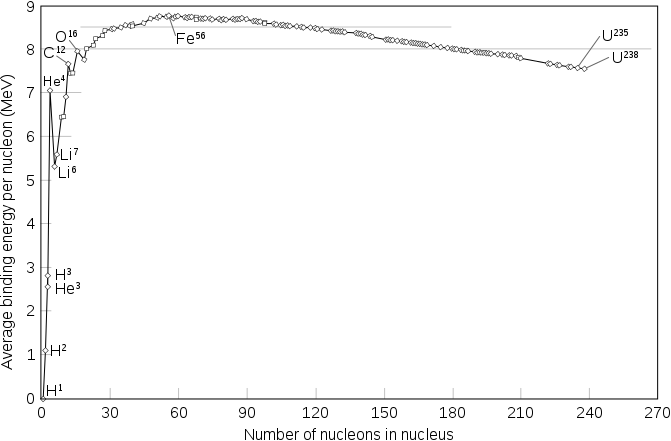
\includegraphics[width=0.9\textwidth, center]{Images/Bindingenergy.png}
\caption{The average binding energy of nucleons against the number of nucleons. This shows that a transition from one light element to another results in a large energy deficit, this is released as energy in a fusion reaction \cite{Fastfission2008BindingNucleon}}
\label{bindingenergy}
\end{figure}

As shown in \autoref{bindingenergy}, lighter elements have far less binding energy per nuclear than heavier elements. This means that, for example, combining two Hydrogen$^{1}$ atoms together will result in a Hydrogen$^{2}$ atom, plus an amount of energy that is released.

\begin{equation}
{^{1}H} + {^{1}H} = {^{2}_{1}H} + {^{1}_{0}e} + {\nu}^{-} + 0.42MeV
\label{eq:H-H}
\end{equation}
\\
The Equation \ref{eq:H-H} is known as a H-H reaction. This process continues but with exponentially decreasing energy release up to iron. Iron is the heaviest element that can be achieved via fusion while still having a positive net energy output. The largest amount of energy from a single reaction can be achieved by fusing two atoms and gaining the largest mass deficit possible. The largest of these being a Deuterium-Tritium (D-T) reaction \cite[p. 430]{Shultis2016FundamentalsEdition.}:

\begin{equation}
{^{2}_{1}H} + {^{3}_{1}H} = {^{4}_{2}He} + {^{1}_{0}n} + 14.1MeV
\label{eq:D-T}
\end{equation}

In this reaction, the neutron inherits the energy as kinetic energy. Conveniently, the D-T reaction also has a high cross section for conditionality combined with a higher probability of the reaction occurring than other considered fuel sources such as H-H or D-D. This was shown in a paper by Lawson \cite{Christopherson1957SomeReactor} to be an inequality to represent the combination between temperature and reaction time. Very few reactors worldwide have attempted a D-T reaction, but those that have suffered significant damage from the high powered neutrons that have been released.

	\section{Tokamak}
Tokamak is an loosely translated acronym for a device developed by soviet Russia in the 1960's, it stands for \textbf{TO}roidal \textbf{CHA}mber with \textbf{MA}gnetic \textbf{C}oils. First results from such a machine were published in 1969 by two Russian scientists, Sakharov and Tamm \cite{Tamm1959TheoryI}. The Russian team managed to produce plasmas of a much higher stability than previously seen, and at temperatures up to 10 times higher than previously achieved. Since then, TOKAMAK development has been progressing, solving one problem at a time, but uncovering many new challenges in the fields of engineering, materials research and plasma physics \cite{Smirnov2010Tokamak19501990}.\\

\begin{figure}[H]

\includegraphics[width=\textwidth, center,angle=0]{Images/Tokamak.jpg}
\caption{A schematic generalised Tokamak showing key features to its operation and function \cite{TokamakEUROfusion}.}
\label{fig:Tokamakschem}
\end{figure}

As shown in \autoref{fig:Tokamakschem} a Tokamak is a collection of Toroidal and Poloidal magnets to generate a helical magnetic field. This is in combination with a central coil which acts as a primary transformer circuit, and the plasma, where moving electrons generate a current acting as a secondary transformer circuit. The magnets create magnetic pressure over the electrons as defined by the Lorentz Force.

In general, the longer that a fusion plasma can be confined (under fusion conditions), the more probability of fusion reactions taking place. There are two main ways to increase confinement time; an increase of radius of a reactor or an increase in magnetic pressure. Magnets are currently approaching the limit of what we can achieve with superconducting technology, so the favoured solution is to increase the size of the reactor. For the purposes of analysing plasma phenomena and performing research a reactor just the right size to fit on all the diagnostics required is adequate, which is the reason behind the building of MAST \cite{Chapman2015OverviewResults}\\

MAST is currently in the process of being upgraded into MAST-U, where is will have many improved features including a new divertor region that allows for more complex plasma configurations and longer path length, which allows the plasma to slow down (and cool down) before striking the divertor plate (\autoref{mastdivertors}, \cite{CulhamCenterforFusionEnergyResearch:Upgrade})

\begin{figure}[H]
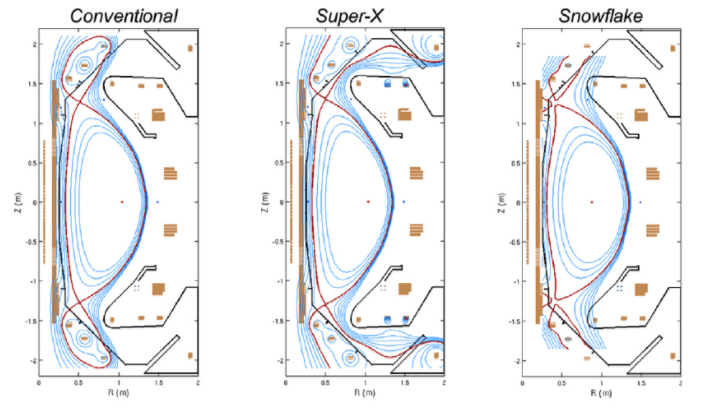
\includegraphics[width=1\textwidth, center,angle=0]{Images/MASTUdivertors}
\caption{MAST-U divertor regions derived by free vacuum boundary calculations. Shows 3 possible new configurations of the magnetic field and ion path passing through the divertor \cite{CulhamCenterforFusionEnergyResearch:Upgrade}.}
\label{mastdivertors}
\end{figure}

	\section{Diagnostics}
There are many forms of diagnostics in a fusion reactor. These can be separated into two different groups; Real Time Diagnostics (Langmuir Probes, Interferometry \cite{Brunner2017}, etc...) and Delayed Diagnostics (Thomson Scattering\cite{Scannell2008DesignMAST}, spectrometry, etc...). Real Time Diagnostics collect data, analyse it and feed it straight back into the system. They are used to make quick changes to try and harness instabilities or to cause a shut down if something goes wrong. Delayed Diagnostics aim to just collect data of a pulse in order for scientists to analyse it at a later time. This is useful for building an understanding of the physical process without sacrificing processing time to analysing data, only collecting it. 
\medskip

One of the main challenges of fusion research, currently, is to limit instabilities generated by Edge Localised Modes (ELMs). This is a disruptive instability that occurs in the edge of a reactor plasma. If ELMs are present in the ITER reactor to the same degree they exist in test reactors, this will catastrophically effect the performance of the machine \cite{Loarte2014ProgressOperation}. These instabilities can seriously damage the reactor wall (particularly divertor plates) as well as causing massive energy losses of the plasma. Ultimately instabilities such as this limit the time that a fusion reactor can run for.
	
	\section{Basic Interferometry}
Interferometry is a method that has been used as a precise measuring tool for many real world applications at many scales such as the detection of gravitational waves \cite{AbbottObservationMerger} all the way down to the measurement of the velocity of blood using Optical Coherence Tomography \cite{Zhao2000Phase-resolvedSensitivity}. As will be discussed in subsequent chapters, it is a powerful diagnostic technique for fusion reactors.
\begin{figure}[H]
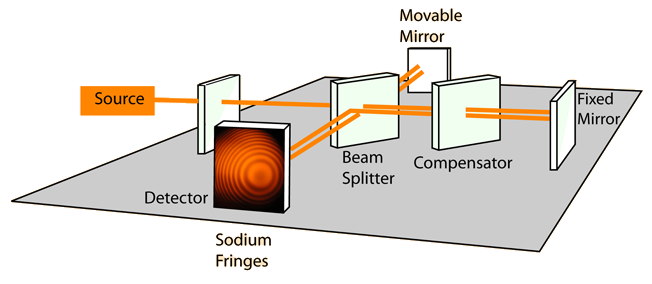
\includegraphics[width=1\textwidth, center,angle=0]{Images/michelsonint.png}
\caption{A standard michelson interferometer experiment where a sodium lamp is used because of its narrow bandwidth. The movable mirror can be translated to produce constructions and de-constructions of interference fringes as can be seen on the viewing plate. The compensator is to account for the additional pass the movable mirror makes through the glass of the beam splitter so both paths are exposed to the same refractive index \cite{Michelsonimage}.}
\label{fig:michelsonint}
\end{figure}

Interferometry was first developed by Michelson and Morley \cite{Michelson1887RelativeEther} as a distance measurement technique. It is the process by which two light waves interact with each other causing interference. In a standard Michelson interferometer, as show in \autoref{fig:michelsonint} , two beams of light go along differing paths and then recombine before being observed. If these paths are of a different length, which can be achieved by using a movable mirror, then a path difference can cause a change in the interference pattern seen. A plane wave can first originally be described as: 

\begin{equation}
E(x,t) = E_{0}\cos{(\omega t - kx)}
	\label{eq:planewave}
\end{equation}
Where $E$ is amplitude, $E_{0}$ is the maximum amplitude of the wave, $\omega$ is the frequency and $k = \frac{2\pi}{\lambda}$, $t$ and $x$ are the positions of the wave in time and 1 dimension, respectively.
Where the overall intensity of the wave can be written as:
\begin{equation}
I \propto <E^{2}>
	\label{eq:intensitypw}
\end{equation}
Since this wave originates from a single light source, but is split into two different beam paths which travel independent distances this can then be described as:
\begin{equation}
E_{1}(x,t) = \frac{E_{0}}{\sqrt[]{2}}\cos{\Big(\omega t - k(2L_{1} - L_{o})\Big)}
	\label{eq:planewave1}
\end{equation}
and
\begin{equation}
E_{2}(x,t) = \frac{E_{0}}{\sqrt[]{2}}\cos{\Big(\omega t - k(2L_{2} - L_{o})\Big)}
	\label{eq:planewave2}
\end{equation}
Where $L_{1}$ and $L_{2}$ are the distances from the beam splitter to each mirror, respectively, and $L_{o}$ is the distance from the beam splitter to the observer.
By combining the waves described by equations \ref{eq:planewave1} and \ref{eq:planewave2} together the superposition of the waves can be described by the following equation at the point of the viewing plate:
\begin{equation}
I_{v} = I_{0} \cos^{2}{\Big(\frac{2\pi}{\lambda}(L_{1} - L_{2})\Big)}
	\label{eq:finalwave}
\end{equation}
This shows us that maxima and minima can be seen when the $\cos^{2}$ function is equal to 1 or 0 and such the following relationships can be stated:
\begin{equation}
Maximum: \Delta L = L_{1} - L_{2} = \frac{n*\lambda}{2}
	\label{eq:fringesmax}
\end{equation}
\begin{equation}
Minimum: \Delta L = L_{1} - L_{2} = \frac{(n+\frac{1}{2})*\lambda}{2}
	\label{eq:fringesmin}
\end{equation}
Where $n = 0, 1, 2, 3, ...$ \\
As such, this shows that the maximum and minimum will occur if there are changes in length of one of the beam paths. The difference between a maximum and a minimum in this system always relates to a distance of a half wavelength, hence, by knowing the wavelength of the light, the displacement of the mirror can be known.\\

	\subsection{Heterodyne Interferometry}
The phase change information caused by a moving mirror can also be gathering by using the doppler effect of light. Unfortunately, currently electrical components cannot measure the temporal resolution with the required sensitivity to see this effect with a single wavelength, so a second is implemented. A heterodyne interferometer is a system that that uses two different wavelength light sources into a single interferometer set up. When the the two different frequencies of light strike the mirror and then interfere, a beat frequency is produced. This beat frequency can be observed on a much smaller frequency scale yet still has the same relationship to the movement of the mirror.

\begin{figure}[H]
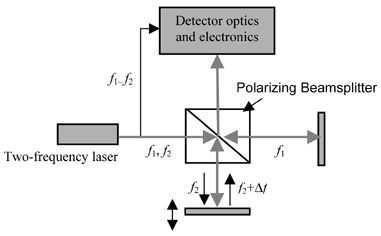
\includegraphics[width=0.8\textwidth, center,angle=0]{Images/heterodyne_system.jpg}
\caption{Schematic of a standard heterodyne displacement measuring system where a reference mirror is used to account for an identical beam path length and the second mirror is the addition of the original frequency to a doppler shift caused by the mirror moving \cite{HeterodyneInterferometer}.}
\label{fig:heterodynesystem}
\end{figure}

As can be seen in \autoref{fig:heterodynesystem}, the fundamental set up is identical to the Michelson Interferometer, but with the addition of a two-frequency laser. This results in the movable mirror causing a frequency shift in the frequency $f_{2}$ by $\Delta f$. This results in the relationship to the beat frequency:
\begin{equation}
f_{beat} = f_{1} - (f_{2} + \Delta f)
	\label{eq:dopplershift}
\end{equation}
Heterodyne interferometry has some clear advantages over homodyne, in that it is less sensitive to laser power fluctuations, ambient light and other noise inputs into the system. Only a single detector is needed to detect the direction and the magnitude of the displacement of the mirror. This does come at the cost that a very precise two-wavelength laser is required for good results along with more complex forms of data handling and electrical components.
    
    \section{Interferometry In Plasma}
Interferometry is a diagnostic tool that has been used in many different fusion reactors around the world. It's purpose is to measure the electron density of the plasma. This can be achieved because the plasma has a refractive index which is proportional to its density, which means the greater the refractive index, the slower the light will travel through it. This simulates the movement of a mirror on a translation stage as used in previous examples of heterodyne and homodyne interferometers. Starting from the dielectric constant of a gaseous medium:

\begin{equation}
\epsilon = 1 + \frac{ne^{2}}{\epsilon _{0} m_{e} (\omega _{0}^{2} - \omega ^{2})}
	\label{eq:DEgas1}
\end{equation}

Where $\omega$ is the wave frequency, n is the number density of some particles of charge e. $m_{e}$ is the mass of the electron and $\omega _{0}$ is the natural frequency of the atom.
Slightly adjust equation \ref{eq:DEgas1} by considering the particles to be electrons, $n_{e}$, to set the value of $\omega_{0}$ to 0 as electrons have no natural frequency, and by substituting in $\omega _{p}^{2} = \frac{n_{e}e^{2}}{\epsilon _{0} m_{e}}$ the equation yields:

\begin{equation}
\epsilon = 1 - \frac{\omega _{p}^{2}}{\omega ^{2}}
	\label{eq:DEgas2}
\end{equation}

The phase velocity, which is the speed of the propagation of the wave can be described by.
\begin{equation}
v_{p} = \frac{\omega}{k}
	\label{eq:phasevelocity}
\end{equation}
Where $k = \frac{2\pi}{\lambda}$, $\omega$ is the frequency of the wave propagating through the plasma.

The phase velocity of a light wave passing through a medium can also have its phase velocity characterised by:
\begin{equation}
v_{p} = \frac{c}{\sqrt[]{\epsilon}}
	\label{eq:phasevelocitylight}
\end{equation}
By re-arranging \ref{eq:phasevelocitylight} for $\epsilon$ and substituting it into \ref{eq:phasevelocity} the following relationship can be found:

\begin{equation}
\epsilon = \frac{k^{2}c^{2}}{\omega ^{2}}
	\label{eq:dielectriccst}
\end{equation}

This equation (\ref{eq:dielectriccst}) can then be set equal to \ref{eq:DEgas2} and solved for $\omega ^{2}$ to find the plasma dispersion relationship.

\begin{equation}
\omega ^{2} = k^{2}c^{2} + \omega _{p}^{2}
	\label{eq:dispersionrelation}
\end{equation}

Since we know that the group velocity of a wave can be characterised by:
\begin{equation}
v_{g} = \frac{\partial \omega}{\partial k}
	\label{eq:groupvelocity}
\end{equation}

By using the dispersion relation it can be said that the phase velocity of high frequency waves that are propagating through the plasma can be described by:
\begin{equation}
v_{p} = \frac{c}{\sqrt[]{1-\frac{\omega _{p}^{2}}{\omega ^{2}}}}
	\label{eq:highfreqprop}
\end{equation}

By differentiating the plasma dispersion relation \ref{eq:dispersionrelation} to find the group velocity and then multiplying the group velocity by the phase velocity:
\begin{equation}
v_{g} v_{p} = \frac{\omega}{k} \frac{\partial \omega}{\partial k} = c^{2}
	\label{eq:groupbyphase}
\end{equation}

Then solving \ref{eq:groupbyphase} for the group velocity yields:
\begin{equation}
v_{g} = \frac{c^{2}}{v_{p}} = \frac{c^{2}}{\frac{c}{\sqrt[]{1-\frac{\omega _{p}^{2}}{\omega ^{2}}}}}
	\label{eq:groupvelocityplasma1}
\end{equation}
Which finally simplifies to the following
\begin{equation}
v_{g} = c \Big(\sqrt[]{1-\frac{\omega _{p}^{2}}{\omega ^{2}}} \Big)
	\label{eq:groupvelocityplasma2}
\end{equation}

This shows that if the plasma frequency is ever less than the frequency of the light that is propagating, the group velocity will become imaginary, hence propagation will not take place - the plasma will be completely reflective. Fortunately, in a reactor the high electron density for all considered wavelengths (Visible - Infrared) results in a transparent medium that has a refractive index proportional to density. This allows the measurement of the density of plasma along a integrated line of sight.\\

One issue which was found in early research is that fusion reactors actually have a mechanical vibration that also incorporates the moving mirror aspect of the previously mentioned interferometers. This will add an additional component to the overall phase shift.

    \subsection{Interferometry In MAST-U}
Currently in MAST-U (Mega Amp Spherical Tokamak - Ugrade) a heterodyne system is in place. This consists of a $CO_{2}$ laser in combination with a HeNe laser integrated with a FPGA system designed by J.K.Brunner \cite{Brunner2017}. So long as the modulation frequency of each of the lasers is known to a high precision, the plasma density can then be derived by a calculation of relative phase between the two paths of the $CO_{2}$ laser. One of the largest limitations to this system is the temperature dependence of the $CO_{2}$ laser. The laser needs to be cooled otherwise it will have slight fluctuations in its output which will affect the phase calculation.\\
Another limitation is the cost of the $CO_{2}$ laser, as it is very expensive and requires a large amount of maintenance. The wavelength of the laser is chosen to have strong interaction with the plasma, but unfortunately it also has strong interaction with human skin and eyes. As a result this laser has very strict safety precautions and requirements that come with its installation.    

\begin{figure}[H]
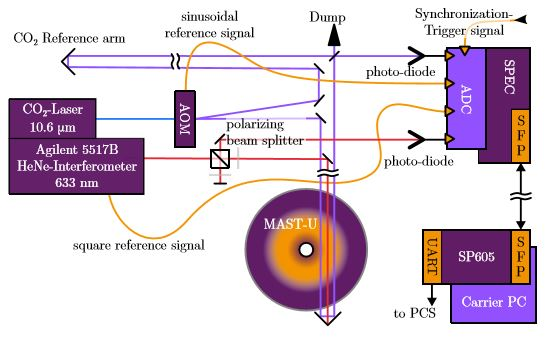
\includegraphics[width=\textwidth, center,angle=0]{Images/mastuint.JPG}
\caption{A schematic of the interferometer currently in place on MAST-U \cite{Brunner2017}.}
\label{MAST-UInt}
\end{figure}


The MAST-U interferometry system as shown in figure \autoref{MAST-UInt} currently uses a $CO_{2}$ heterodyne system in combination with a $HeNe$ homodyne system. Both beams enter the plasma, passing through the bulk and perform a double pass due to collision with the retro reflector, an 80kg granite sphere. In this system an Acousto-Optical Modulator (AOM) is used to generate an additional frequency that is used to modulate the frequency of the $CO_{2}$ laser, in this case by 40MHz. This allows the $CO_{2}$ laser to act as two independent wavelengths to fulfil the frequency shift requirement of equation \ref{eq:dopplershift}.

    \subsection{Measuring Electron Density using Interferometry}
In a plasma the optical path in a double pass interferometer (passing through the plasma twice) can be calculated according to the following equation \cite[p.~26]{Brunner2017} :

\begin{equation}
	\Delta s = 2 \int_{0}^{L} [N_{air} - N_{pl}(l)]dl \approx 2 \int_{0}^{L} \Bigg[1 - \sqrt[]{1-\frac{\omega_{pe}^{2}}{\omega^{2}}}\Bigg]
	\label{eq:opticalpathint}
\end{equation}

Where $N_{pl}$ denotes the plasma's refractive index that already includes the visible light approximation. $N_{air}$ is the refractive index of air. $\omega$ is the frequency of the laser and $\omega_{pe}$ is the frequency of the plasma. This can then be expanded by assuming that the plasma frequency is much less than the frequency of the laser to achieve:

\begin{equation}
	\Delta\phi_{pl} = \frac{\lambda e^{2}}{2 \pi c^{2} \epsilon_{0} m_{e}} \int_{0}^{L} n_{pl} (l) dl
	\label{eq:plasmaphase}
\end{equation}

\begin{equation}
	\int_{0}^{L} n_{pl} (l) dl = \frac{2 \pi c^{2} \epsilon_{0} m_{e}}{\lambda e^{2}} \Delta\phi_{pl} = \frac{2 \pi}{\lambda n_{c}} \Delta\phi_{pl}
	\label{eq:phaseintegral}
\end{equation}
\\
Where $\Delta\phi_{pl}$ is the phase difference between the two interferometer arms. $\lambda$ is the wavelength of the laser used. e and c are the electron charge and the speed of light in a vacuum, respectively. $\epsilon$ permittivity of free space and $m_{e}$ is the mass of the electron. $n{pl}$ is the density of the plasma, which in an ideal hydrogen plasma can be defined entirely by the density of the electrons as the Debye length of the ions is on too large a scale for the measurement to make a contribution. 

This now gives a viable way to calculate the change in phase of a laser passing through plasma. Providing the precise distance of the beam path within the reactor is known with a precision to the order of the wavelength of the laser. Unfortunately the vibration of the machine causes this value to fluctuate causing uncertainty in the phase. For this reason two different colour lasers that follow the same beam path must be implemented. One must interact strongly with the plasma and the wall, the other must interact weakly with the plasma and strongly with the wall.
	
    
    \subsection{Measuring Electron Density Accounting for the Vibration of the Wall}
There are two causes for a change in optical path in an interferometer system; a change in refractive index, or a change in physical length (vibration). Both of these are occurring simultaneously within a reactor and so both have to be accounted for. This can be done by considering total phase change to be the superposition of the vibrational phase change and the phase change due to the refractive index (plasma).

\begin{equation}
	\Delta\phi = \Delta\phi_{pl} + \Delta\phi_{vib}
	\label{eq:superposphasediff}
\end{equation}

Where $\phi$ is the total phase change, and $\Delta\phi_{pl}$ and $\Delta\phi_{vib}$ are the phase changes caused by the plasma and the vibrations of the machine respectively. Because a change in length causes a linear change in phase for a laser that interacts strongly with the wall, the change in phase due to the vibrations can easily be characterised by a change in length divided by the wavelength of laser sensitive to vibrations in the machine, such that:

\begin{equation}
	\Delta\phi_{vib} = \frac{2\pi}{\lambda} \Delta L
	\label{eq:vibphasediff}
\end{equation}

Combining the equation derived for a single laser passing through the plasma \ref{eq:plasmaphase}, the superposition of the vibration and plasma phase \ref{eq:superposphasediff} and the vibrational phase \ref{eq:vibphasediff} a complete equation for phase shift can be formed:

\begin{equation}
	\Delta\phi = \frac{\lambda e^{2}}{2 \pi c^{2} \epsilon_{0} m_{e}} \int_{0}^{L} n_{pl} (l) dl + \frac{2\pi}{\lambda} \Delta l
	\label{eq:heterophasediff}
\end{equation}

Since the relationship between the phase of the two lasers observe an inversely proportional relationship it is possible for only density information $n_{pl}$ to be extracted. This can be done by making $\Delta l$ the subject:

\begin{equation}
	\Delta l = \frac{\Delta\phi\lambda - \frac{\lambda^{2} e^{2} \int_{0}^{L} n_{pl} (l) dl }{2 \pi c^{2} \epsilon_{0} m_{e}}}{2 \pi} 
	\label{eq:deltal}
\end{equation}

and substituting in for the classical electron radius $r_{ce} = \frac{e^{2}}{2 \pi c^{2} \epsilon_{0} m_{e}}$ gives an equation of the form:

\begin{equation}
	\Delta l = \frac{\Delta\phi\lambda - \lambda^{2} r_{ce} \int_{0}^{L} n_{pl} (l) dl}{2 \pi}  
	\label{eq:deltalrce}
\end{equation}

By now considering two lasers of different wavelengths, $\lambda _{1}$ and $\lambda _{2}$, that follow identical beam paths and there for the same exposure to mechanical vibrations, $\Delta l$ will be equal. These two equations can then be equated:

\begin{equation}
	\frac{\Delta\phi _{1}\lambda _{1} - \lambda _{1}^{2} r_{ce} \int_{0}^{L} n_{pl} (l) dl}{2 \pi}  = \Delta l = \frac{\Delta\phi _{2}\lambda_{2} - \lambda _{2}^{2} r_{ce} \int_{0}^{L} n_{pl} (l) dl}{2 \pi}  	\label{eq:deltalequate}
\end{equation}

and then solved for the line integrated plasma density, $\int_{0}^{L} n_{pl} (l) dl$, yielding:

\begin{equation}
\int_{0}^{L} n_{pl} (l) dl = \frac{1}{r_{ce}} \frac{\Delta\phi _{2} \lambda _{2} - \Delta\phi _{1} \lambda _{1}}{\lambda _{2}^{2} - \lambda _{1}^{2}}	
    \label{eq:LIPD}
\end{equation}

As a result of equation \ref{eq:LIPD}, the line integrated plasma density can be calculated from two values of change in phase using two different wavelengths. This takes into account mechanical vibrations, which are factored into $\Delta \Phi$ by equation \ref{eq:superposphasediff}.

	\section{Field Programmable Gate Array's (FPGA's)}
FPGA's are a simple and effective way to collect and analyse data. They have numerous advantages over standard processing devices as they are designed to compute a single pre-programmed task, as unlike a Central Processing Unit (CPU) which is designed to use logic to solve a specific task. The use of an FPGA is becoming more common in fusion applications as the need to perform real time filtering \cite{Naylor2010AnMAST} and processing on data is becoming a greater concern for plasma control systems to allow the safe operation of reactors. Many different forms of FPGA's have been used in the fusion industry for real time application.
	\subsection{Red Pitaya}
    
The Red Pitaya (RP) \cite{Leban2014RedManual} is a micro controller that has built in FPGA capabilities. FPGA's are notorious for being difficult to program as they are intrinsically complicated. The stand out function of a FPGA is the way it processes information. It can perform many tasks in parallel pipelined processing i.e. performing the same operation on many data sets. The number of parallel pipelines that can be implemented depends entirely on the hardware limitations of the FPGA. This often means that the limiting factor of the speed at which a RP can process data is the speed at which you can transmit data to it. This gives FPGA's a large advantage over conventional computers when it comes to real time data applications. This is simplified by Koheron by designing software for the RP to run, which includes an oscilloscope and spectrum analysis software as well as control of the laser's modulation frequency and current, through a simple interface.

\begin{figure}[H]
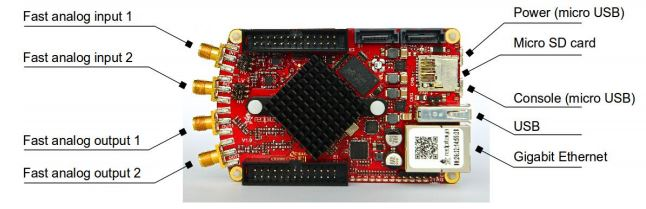
\includegraphics[width=0.9\textwidth, center,angle=0]{Images/RP.JPG}
\caption{The Red Pitaya showing all the connected ports. Each of the analogue ports can sample at 125MHz \cite[p.~7]{Leban2014RedManual}.}
\label{RP}
\end{figure}

\begin{table}[H]
	\setlength\arrayrulewidth{1pt}
    \rowcolors{2}{gray!25}{white}
    \begin{tabular}{ c c c c } 
        Name & Type & Connector & Description\\
        \hline
        IN1/IN2 & Input & SMA-F & RF input(High-Z, 1M$\Omega$ // 10pF\\[1pt]
        OUT1 / OUT2 & Output & SMA-F & RF output (50$\Omega$)\\[1pt]
        Ethernet & Full Duplex & RJ45 & 1000 Base-T Ethernet Connection\\[1pt]
        USB & Full Duplex & A USB & Used for standard USB Devices\\[1pt]
        Micro USB (Console) & Full Duplex & Micro B USB & Used for console connection\\[1pt]
        Micro USB (Power) & Input & Micro B USB & 5V / 2A power supply\\[1pt]
        Micro SD & Full Duplex & Micro SD slot & Micro SD memory card\\
    \end{tabular}
    \caption{Full Specifications of the Red Pitaya's input/output ports. Both fast analogue inputs and fast analogue outputs operate at 125MHz per channel \cite[p.~7]{Leban2014RedManual}.}
    \label{RPspec}
\end{table}

\section{Koheron} 
Koheron have developed a laser board which connects to the Red Pitaya that can simulate the AOM in \autoref{MAST-UInt}. It does this by using a fiber optic cable to generate a frequency modulation that results in a beat frequency \cite{KoheronAmplitudeKoheron}. Initial investigations at CCFE \cite{Hickling2017InvestigationMAST-U} have shown this method to show a strong interference pattern and the use of the RP and Koheron software is easy and accessible. There is a large amount of support and development occurring constantly so any new problems found can be fixed. In this investigation it was shown that the basic interferometer set up from Koheron is not currently sensitive enough to physical vibrations on the order of 10's of KHz. It was found that this may be due to the lack of any high order modulation of the laser due to an Acousto-Optical Modulator, as discussed by J. Brunner \cite[p. ~29]{Brunner2017}. Due to this, an AOM may be required for detection of the required beat frequency, however the benefits of this system are still apparent over the use of a $CO_{2}$ laser system. Many aspects of this system will need to be characterized before it can be considered as a functional system for the measurement of density.

%----------------------------------------------------------------------------------------
%	Aims and Objectives
%----------------------------------------------------------------------------------------

\chapter{Aims and Objectives}
The literature review has outlined key goals in the development and testing of a new interferometer diagnostic device. It is known that the device currently installed on MAST-U, while effective, has significant drawbacks. It has been shown by previous research \cite{Hickling2017InvestigationMAST-U} that the Red Pitaya / Koheron based system can measure the phase difference of a heterodyne system. It is still unknown if it can do this with enough precision to make it a valid candidate to the replacement of the interferometry system currently on MAST-U. In an attempt to characterise a new system for installation tests will need to be run to assure that the phase noise, which will ultimately dictate its effectiveness, will need to be on the order of approximately 10 milliRads in order to detect any useful densities. As such, this project will be to characterise and minimise any noise that is in this system. \\

\begin{center}
\begin{ganttchart}{1}{12}
  \gantttitle{Aims and Objectives (Weeks)}{12} \\
  \gantttitlelist{1,...,12}{1} \\
  \ganttbar{Task 1}{1}{1} \\ %Lit Study
  \ganttlinkedbar{Task 2}{2}{3} \\ %Analyse Error in free space (repeat tom)
  \ganttlinkedbar{Task 3}{4}{5} \\ %Analyse error in fiber
  \ganttlinkedbar{Task 4}{6}{7} \\ %increase fiber length to 25m and repeat task 3
  \ganttlinkedbar{Task 5}{8}{9} \\ %Test on plasma at NTU?
  \ganttlinkedbar{Task 6}{10}{12} %Documentation for CCFE and NTU
%  \ganttmilestone{Milestone}{7} \ganttnewline
  %\ganttlink{elem1}{elem2}
  %\ganttlink{elem1}{elem3}
  \end{ganttchart}
\\
\end{center}
This Gantt chart to show the tasks involved in the execution of this project. Details about each individual task can be seen in \autoref{tbl:tasks}.
\begin{center}
\begin{table}[H]
	\setlength\arrayrulewidth{1pt}
    %\rowcolors{2}{gray!25}{white}
    \begin{tabular}{|p{1cm}|p{2.5cm}|p{9cm}|p{1.5cm}|}
    			\hline
    	        Task & Objective & Description & Duration (Weeks)\\
                \hline
                1 & Literature Study & Background Study into heterodyne interferometer systems making comparisons of the benefits and drawbacks including the mathematical frame work for plasma interferometry. & 1\\
                \hline
                2 & Analyse the error sources using free space& Analyse standard deviation of different phase noise sources while adjusting the length of exposed free space. Decide if the laser will be appropriate for use in current state on MAST-U.  & 2\\
                \hline
                3 & Analyse the error sources using fiber optics& Compare results to free space using the interferometer system described in J. Brunner's Thesis, \autocite{Brunner2017}. Attempt to achieve a phase error of 3$mRad$ or less.& 2\\
                \hline
                4 & Repeat Task 3 with varying length fibers (up to 25m)& Analysing the error sources using a much longer fiber to better simulate the beam paths that would be used on MAST-U. Attempt to maintain the same error. & 2\\
                \hline
                5 & Test on plasma device & Test the system on an actual plasma device to see the variation in density to attempt to characterise the plasma. & 2\\
                \hline
                6 & Docume- ntation & Full documentation of work performed and results obtained for use by CCFE and also for handing in of dissertation. & 3\\
        \hline
	\end{tabular}
    \caption{Detailed evaluation of each task that must be undergone for successful completion of the project.}
    \label{tbl:tasks}
\end{table}
\end{center}

%----------------------------------------------------------------------------------------
%	Methodology
%----------------------------------------------------------------------------------------
\chapter{Experimental}

%----------------------------------
%	Phase Noise
\section{Phase Noise}
Phase noise is the major component that ultimately describes the resolution to which differences in the phase can be detected. Phase noise has many different contributing factors in the system and all of the factors that contribute towards phase (discussed in 2.5) also have contributing factors to phase noise. Since the calculations that this system will eventually lead to are calculations of the density, which is measured by the phase, any error in phase measurement affects the resolution of density measurement.

\begin{figure}[H]
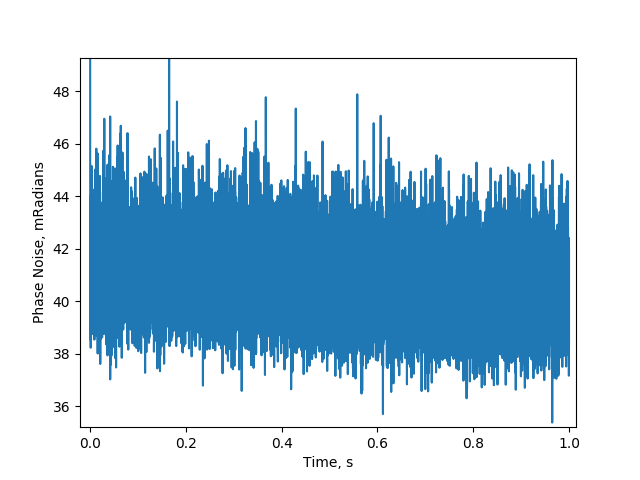
\includegraphics[width=0.8\textwidth, center,angle=0]{DImages/Phase_Noise_for_Scene_shot_13_with_bandwidth___1000_Date_20180323.png}
\caption{Phase noise for shot 13 taken on 23/03/2018 with a bin width of 1000 therefore corresponding to a frequency bandwidth of 20KHz. It can be seen that this has a large spread of data across several mRad and many peaks at varying heights.}
\label{fig:phasenoise1}
\end{figure}
As can be seen in \autoref{fig:phasenoise1} phase noise just appears on a phase difference graph as white noise. This limits our ability to only see detail that results in phase changes greater than this noise. Using the equation for plasma density \autoref{eq:LIPD} we can see that the smaller phases that can be detected precisely results in smaller density changes. The relationship between phase noise and density is linear, as following the plot shown in \autoref{pn_density}.

\begin{figure}[H]
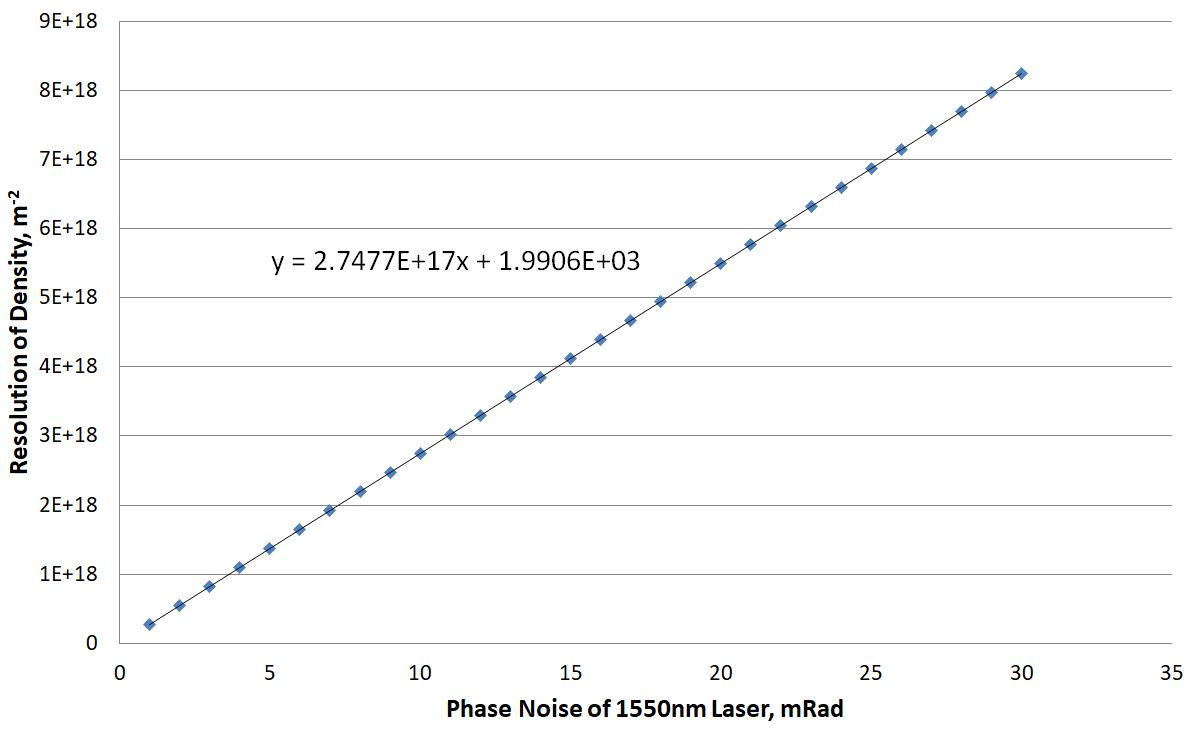
\includegraphics[width=0.9\textwidth, center,angle=0]{DImages/pn-density-relationship.JPG}
\caption{Relationship between Phase noise of the 1550nm interferometery path and the resolution of the phase by using \autoref{eq:LIPD}.}
\label{pn_density}
\end{figure}

The phase noise in general is a very high frequency form of noise, that is caused mostly by the mixing of slight variations in frequency caused by the inherent property of laser line width.
Since the equation that dictates the resolution of a density measurement is linear, there is no optimal phase noise to achieve, it is simply a fact of minimising the phase noise so as to achieve the best resolution. 

The phase noise can be characterised by the standard deviation of the measured phase. By taking this standard deviation over a range of bandwidths certain frequencies can be isolated from the system. This will, by default reduce the calculated phase noise, but will not affect the density resolution as that is a holistic calculation that can be characterised by the phase noise, not directly calculated. If the dataset of the phase difference exists with little to no variation from in the Y-Axis except for that induced by vibrations then a simple standard deviation calculation would give a very good idea of the limitations of the resolution of the phase. As is discussed in later chapters there is an inherent drift seen in nearly all shots taken which would result in the standard deviation including this drift, which isn't an accurate representation of the phase. As a result it is much better to bin the data and perform a standard deviation of each bin to minimise the effect of this drifting response. The average of the standard deviation of each of these bins will more accurately reveal the resolution of the phase and therefore what would be expected in the resolution of the density.//

Noise that can be detected by a phase shift comes in two distinct flavours; low frequency or "one over f" noise, and high frequency or "white noise". These two different types of noise can be distinguished on an FFT plot of the dataset which shows a distinct change in gradient. The point at where this change in gradient occurs is important to give an idea of the performance of the system.

\section{Experimental Design}

%-------------- Summer Work ------------------------------

As discussed in \cite{KoheronAmplitudeKoheron} a frequency modulation can also be induced into a system by the addition of a small fiber optic extension to an arm of a interferometer. This can be seen in \autoref{koheronfmod}.

\begin{figure}[H]
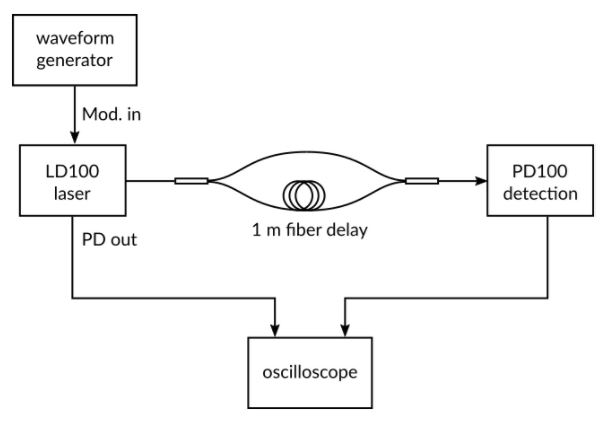
\includegraphics[width=0.9\textwidth, center,angle=0]{DImages/koheronfmod.JPG}
\caption{Experiment designed by Koheron where a 1m fiber extension can be used to create a frequency modulation when interfered with the original light source.}
\label{koheronfmod}
\end{figure}

This system is attractive as it removes the requirement of needing an AOM to modulate the frequency of the scene interferometer laser. Unfortunately, preliminary testing has shown that the phase noise of this system is too high to detect a 10KHz vibration produced by a speaker \cite{Hickling2017InvestigationMAST-U}.

\subsection{Optical Components}

\subsubsection{Koheron Laser}
The 1550nm laser \cite{KoheronLaserV1} is provided by Koheron and is designed to have a maximum output of 3mW. This results in the laser being listed as class 1 and this confirms its safe use with a minimal amount of safety equipment or restrictions. The laser does has a line width of 6MHz which may prove to be too large for this application, as such the scope of this chapter will be to discuss the suitability of this component.

\subsubsection{fiber Optic Splitters}
Used to split an incoming electromagnetic wave \cite{1x2Koheron} where approximately 50$\%$ of the light passes down each of the two fibers. This is imperative for the system as it makes the laser common among all parts of the beam path. This means that if the laser is exposed to any kind of internal fluctuation it is common and therefore should not significantly affect the results.

\subsubsection{Circulator}
The circulator \cite{FiberKoheron} is sources by Koheron and it's function is to allow exit and re-insertion into the fiber system from the same point within the system. It manages to achieve this with near 100$\%$ efficiency. It does this by a module which is sensitive to the direction of the incident light, such that light can travel from port 1 to port 2 and from port 2 to port 3, but not from 1 to 3. This allows for the sending of the light out into free space and then return it back into the fiber system.

\subsubsection{Collimator}
The appropriate collimator \cite{Air-SpacedSMA} for 1550nm is employed so collimate the light once it exits the fiber. This is important as if the light is uncollimated the losses due to divergence across free space become significant. The selected collimator has a divergence angle of 0.016 degrees. Across 2m this will result in a 3.2cm divergence of spot radius, which will be very significant. In larger free space systems a correction lens will need to be applied.

\subsubsection{Retroreflector}
A standard retroreflector (sometimes called a "Corner Cube") is employed to reduce the difficulty of alignment in free space. It functions by having 3 highly reflective surfaces that all meet perpendicularly to form a vertex, this resembles in internal corner of a cube. All light that strikes any one of these reflective surfaces will be sent back on a beam path that is parallel to the incident beam.

\subsubsection{Acousto-Optical Modulator}
The AOM \cite{Sell1550MODULATOR} chosen for this system is a  T-M040-0.5C8J-3-F2S designed to modulate the signal of the input 1550nm signal by 40MHz. It has a low insertion loss of 2.5dB and up-shifts the frequency of the incoming light by 40MHz. This results in a wavelength change of $~0.32pm$.

\subsubsection{PD100 Photo detector}
The PD100 designed by Koheron \cite{KoheronPD100Photodetector} is a low noise photodetector that has a maximum input of 1.5mW. This signal can then be output electronically by an SMA connection for data processing.

\subsubsection{FPGA Digitisation Board}
The data collection is processed by a SPEC board and a SP605 as designed by Jakob Brunner as the aim of his thesis \cite{Brunner2017}. The SPEC board takes an input of the PD100 and send the data to the SP605 using the FPGA process of Xilybus. The SP605 then performs a CORDIC phase algorithm to extract useful information from the signal which includes the phase. The SPEC board requires 2 signals, a scene and a reference. The scene is provided by the portion of the interferometer that passes through free space, and the reference is provided by the signal generator (AOM Driver). It then calculated the difference between the phase of these two signals.

\subsubsection{AOM Driver}
The AOM is driven by the use of a Red Pitaya \cite{Leban2014RedManual} which can generate a 40MHz signal for the use of the modulation. It does this through the use of 1 of its 2 Digital to Analogue converters which can output at 125 MHz. This provides the signal to the AOM and also to the reference.

\subsubsection{Laser Diode}
To compare and contrast the strengths and weaknesses of the Koheron system it will have to be compared to another laser in an identical set up. The laser chosen is an SFL1550S - 1550 nm with a butterfly connection \cite{ThorlabsFC/APC}. The benefit of this laser over the Koheron is that this only has a 50KHz (Max 100KHz) line width.

\subsubsection{Laser Driver}
This laser, being a butterfly connection has to be driven by some current control unit, to which the Thorlabs compact laser diode driver was chosen \cite{CompactPackages}. This driver was chosen due to its precise current control and the benefit of including temperature control to a precision of 0.005 Kelvin. As temperature increase so does the line width of the laser, which can result in some negative effects on the phase.

%-------------- Addition of AOM ------------------------------
\subsection{Optical Configurations}
In order to improve the phase noise an AOM has been employed into the system to measure the effectiveness of the 1550nm laser provided by Koheron. With the introduction of the AOM \cite{Sell1550MODULATOR} as seen in \autoref{fig:intconfig1} half of the signal of the laser is modulated by a clean 40MHz sine wave which is produced by a signal generator. It is necessary for the stability of the modulation to be high as the detected wave has a strong dependence on a stable beat frequency defined by the mixing of two different frequency signals.

\begin{figure}[H] 
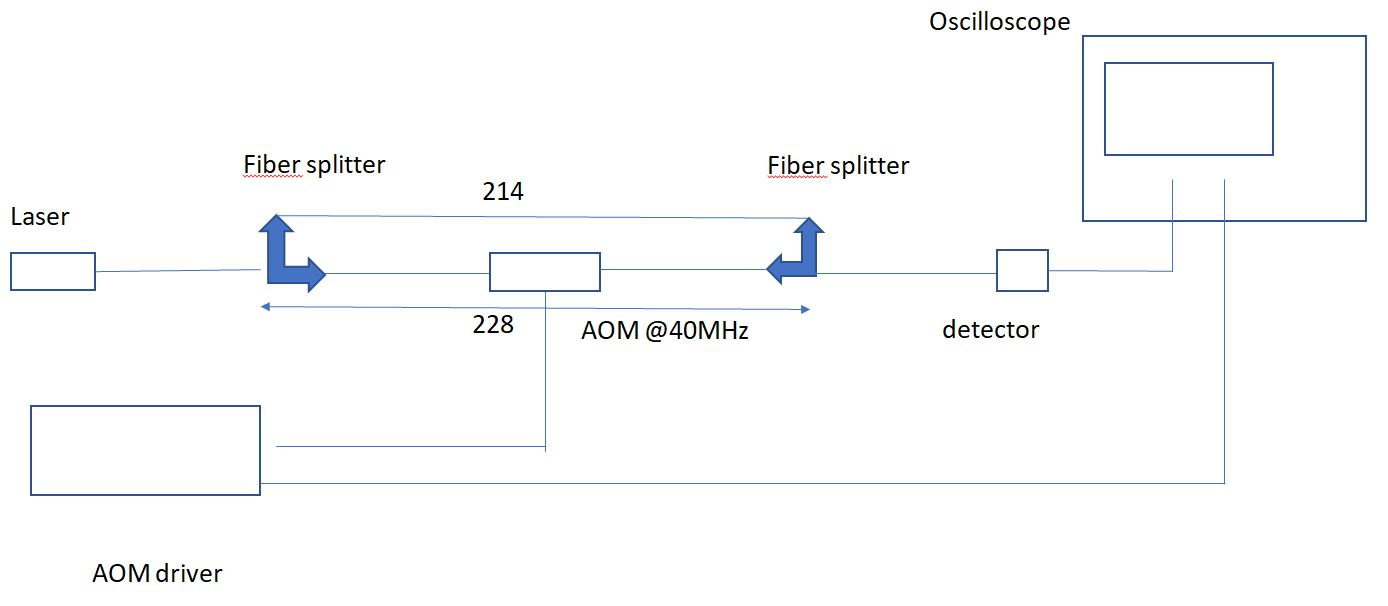
\includegraphics[width=0.9\textwidth, center,angle=0]{DImages/intconfig1.JPG}
\caption{Experimental set up designed to test the noise present in the phase using only fiber optics.}
\label{fig:intconfig1}
\end{figure}

While the fiber only set-up gives a good representation of the expected phase noise of the system it does not mimic what we want the final system to look like. For this a free-space portion will have to be included in one of the arms of the interferometer as shown in \autoref{fig:intconfig2}. This will cause the system to become sensitive to mechanical vibrations as described by \autoref{eq:vibphasediff}.


%-------------- Free Space Setup ------------------------------
\begin{figure}[H] 
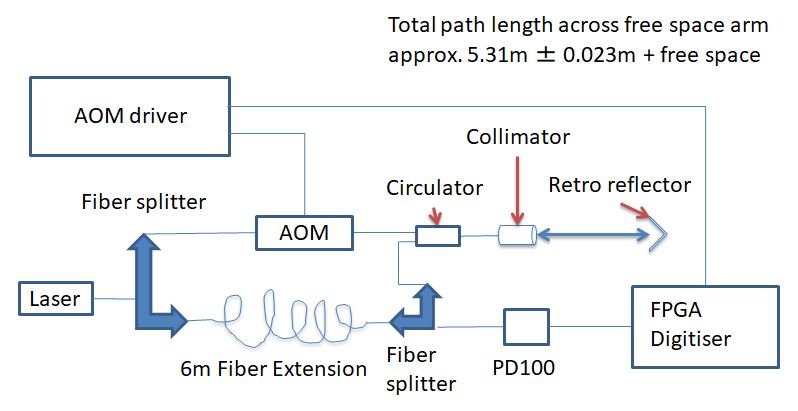
\includegraphics[width=0.9\textwidth, center,angle=0]{DImages/intconfig2.JPG}
\caption{Experimental set up designed to test the noise present in the phase while employing a free space portion of the path which allows the measurement of some medium with refractive index as well as physical vibrations.}
\label{fig:intconfig2}
\end{figure}

As will be explained in later sections a drift of phase difference can be seen, as such it was important to instead of comparing the moving phase of the interferometer to the stationary phase of the AOM driver, to instead compare it to the moving phase of a reference interferometer as shown in \autoref{fig:intconfig3}. The idea is that any drift caused by the laser or by temperature fluctuations within the system will be common in both interferometers, and so these will cancel out when the phase difference calculation is performed. 
%-------------- Fiber Reference ------------------------------
\begin{figure}[H] 
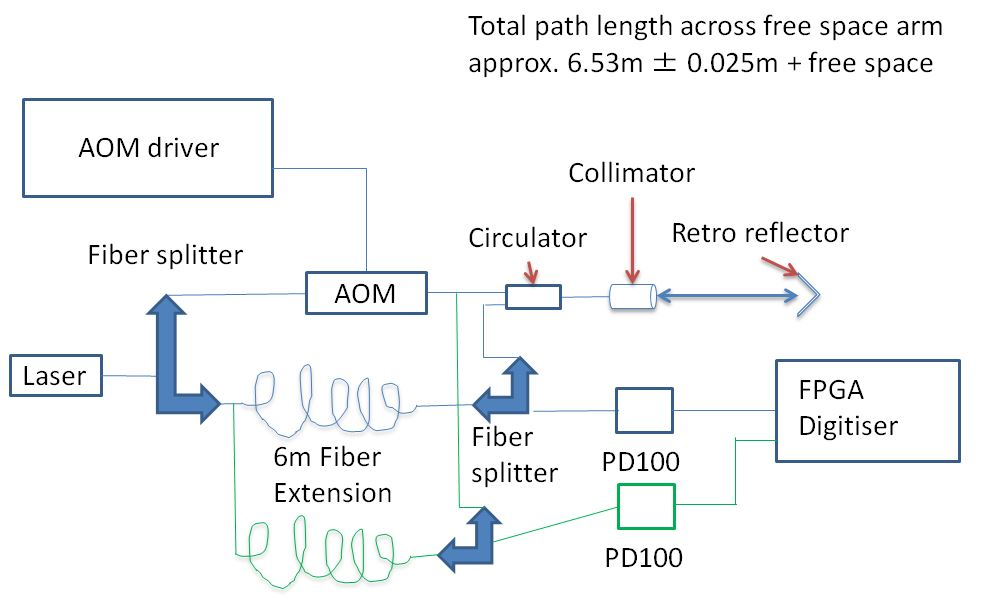
\includegraphics[width=0.9\textwidth, center,angle=0]{DImages/intconfig3.JPG}
\caption{Interferometer system with the laser as a common signal between both the scene and the reference arms. This causes any fluctuations in the laser to be seen on both detectors and then cancelled out in the difference calculation.}
\label{fig:intconfig3}
\end{figure}

The final configuration that has been explored is once which compares the signals of each interferometer to the AOM driver signal as shown in \autoref{fig:intconfig4}. This is designed to attempt to show if there is a dominant cause of phase drift in one interferometer, and exactly to what extent these two interferometer arms actually have correlation.
%-------------- Ref and Scene Drift ------------------------------
\begin{figure}[H] 
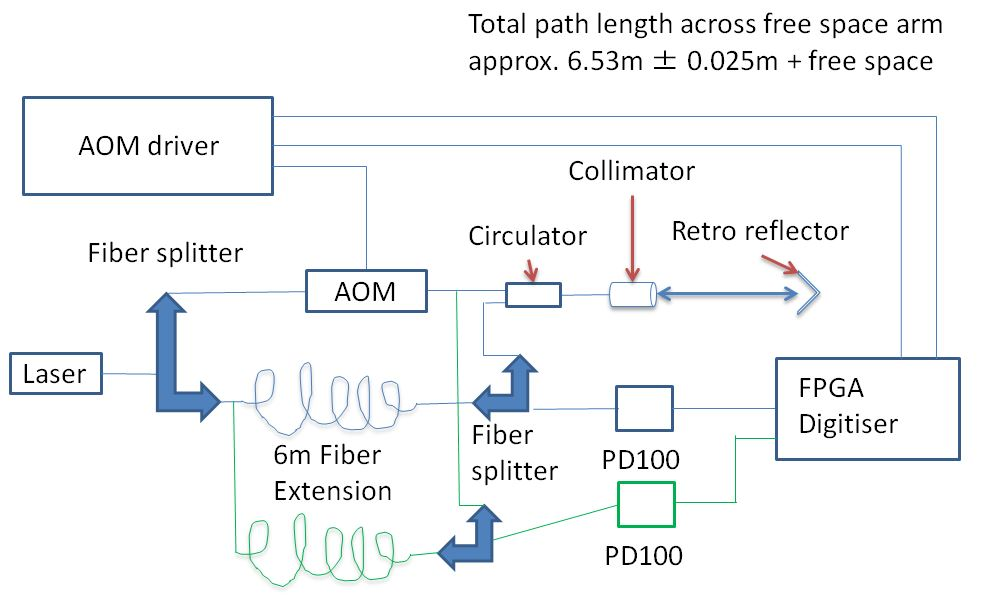
\includegraphics[width=0.9\textwidth, center,angle=0]{DImages/intconfig4.JPG}
\caption{Combines the scene interferometer with the AOM driver signal and also the reference interferometer with the AOM driver signal. This allows the viewing of the individual movement of each set in an attempt to try and characterise the slow drift.}
\label{fig:intconfig4}
\end{figure}



%----------------------------------------------------------------------------------------
%	Red Pitaya
%----------------------------------------------------------------------------------------

\chapter{Use of Koheron Laser}
\section{Overview and Operation}
The Koheron laser is a cheap and effective laser diode which is capable of producing a 1550nm wavelength with a 3MHz linewidth. The laser power is inherently low (Maximum 3mW) which makes it a safe system to operate with no restrictions. The laser has been tested with all 3 set ups shown above (\autoref{fig:intconfig2}, \autoref{fig:intconfig3} and \autoref{fig:intconfig4}) including the original set up to test the modulation of the fiber \autoref{fig:intconfig1}. It is to be noted that the laser is not temperature cooled and appears to show a period of multi-mode operation at an input current of 25mA which can be seen in the fft as shown in \autoref{fig:singlemode_multimode}. By running at a different current, e.g. 30mA this aditional frequency contribution is no longer present.

\begin{figure}
  \begin{subfigure}{.5\textwidth}
    \centering\captionsetup{width=.90\linewidth}
    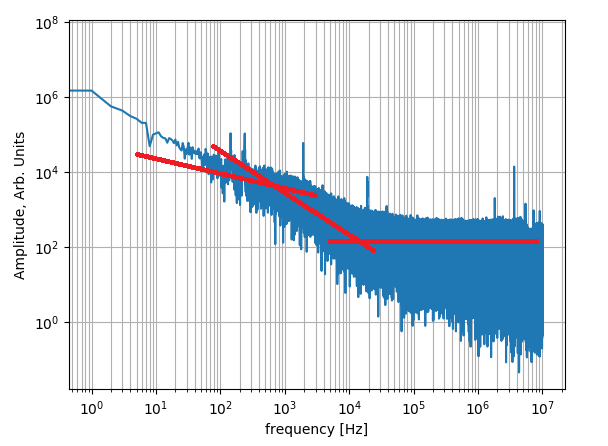
\includegraphics[width=\textwidth,angle=0]{DImages/FFT_for_shot_8_Date_20180323.png}
    \caption{Shot 8 taken on 23/03/18 at 25mA shows three distinct gradients can be seen as indicated by the red lines. This shows that there are multiple frequency responses at this particular setting for the laser.}
  \end{subfigure}
  \begin{subfigure}{.5\textwidth}
    \centering\captionsetup{width=.95\linewidth}
    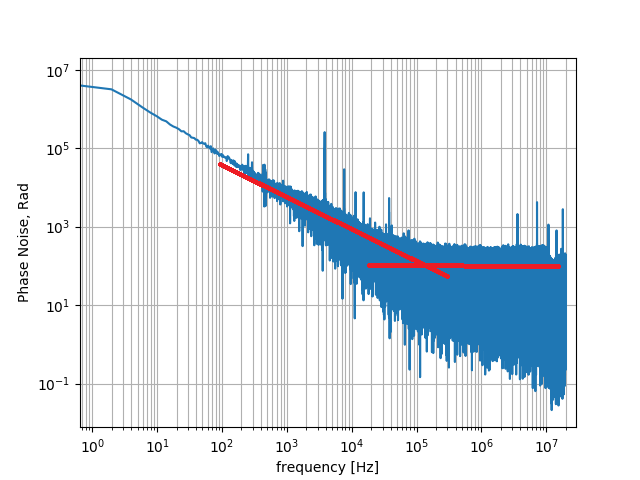
\includegraphics[width=\textwidth, angle=0]{DImages/FFT_for_shot_6_Date_20180412.png}
    \caption{Shot 6 taken on 12/04/18 at 30mA shows only two distinct gradients. This is in line with what we expect to see from single mode operation as there is contribution only from a single set of noise.}
  \end{subfigure}
\caption{FFT's from two different shots running at two different currents both using the Koheron laser board. (a) shows the laser being operated by 25mA showing multimode operation, (b) shows the laser being operated at 30mA showing single mode operation. }
\label{fig:singlemode_multimode}
\end{figure}


The operation of the laser is very simplistic as it runs entirely within the Koheron web client. The web client allows the laser current to be chosen to a precision of $\pm 0.005A$ and also allows the input of modulation into the system (though this feature will not be used for the purposes of these tests). As a result to avoid multi mode operation a current of 30mA for all tests is chosen, this is to also maximise signal for detection purposes.
%----------------------------------------------------------------------------------------
%	Results
%----------------------------------------------------------------------------------------
\section{Results} \label{Section:RP_Drift}

\begin{figure}[H]
\autoref{fig:pdshot5d20180423} shows a standard phase difference for a shot taken by the Koheron laser. The phase difference shows a significant amount of phase drift as it moves from ~-2.6 Radians down to -3.1 Radians with little to no change in amplitude. In a plasma exposed system this would represent a density change within the fiber.

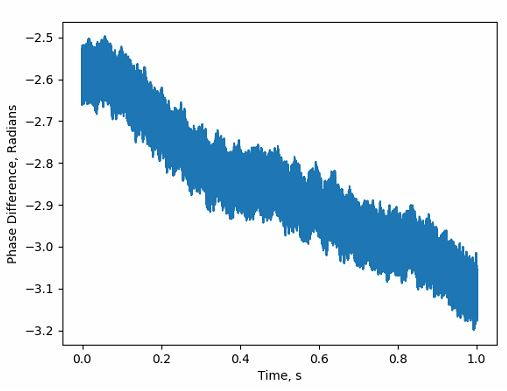
\includegraphics[width=0.9\textwidth, center,angle=0]{DImages/PD-shot-5-date-20180423.JPG}
\caption{Phase difference of Shot taken on as analysed by Jakob Brunner's evaluation code.}
\label{fig:pdshot5d20180423}
\end{figure}

This can be clearly seen on other shots and the amount that it drifts by changes drastically. As can be seen in \autoref{fig:PD-shot-2-20180323} this shot actually drifts in phase difference by an entire radian. This is the upper limit of the amount of drift that is commonly seen from shot to shot. From time to time turning points (seen in \autoref{fig:PD-shot-2-20180411} in which drifts can be seen which implies that this is some kind of fluctuation rather that just some constant change in a single direction. It has changing gradients and amplitudes so it is impossible to predict from shot to shot.
\begin{figure}[H] 
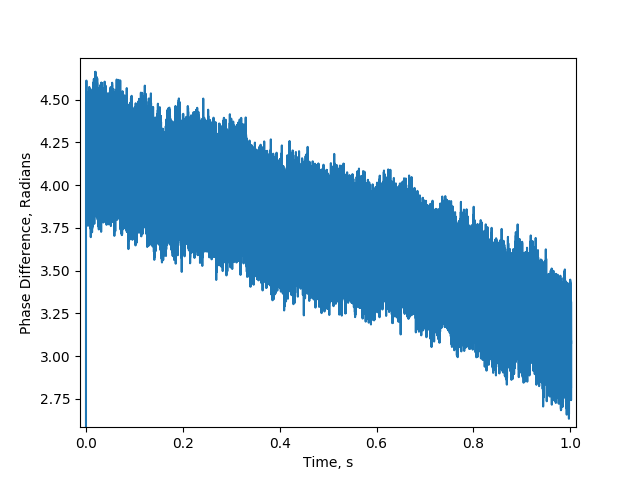
\includegraphics[width=0.9\textwidth, center,angle=0]{DImages/Phase_Difference_shot_2_Date_20180323-1.png}
\caption{Phase difference of shot 2 taken on 2018-03-23. Drift is clearly visible on a scale of about 1 Radian.}
\label{fig:PD-shot-2-20180323}
\end{figure}

As can be seen in \autoref{fig:PD-shot-2-20180411} turning points are frequent. By placing a warm object near one of the interferometer arms a phase shift can be seen. As seen on an oscilloscope a increase in temperature causes a forward shift and a decrease causes a reverse shift. It is possible that these drifts are caused by changes in temperature in the fibers which would result in random frequencies in the range of 0.2-1.2Hz \cite{Melikov1997AirRooms}.
\begin{figure}[H] 
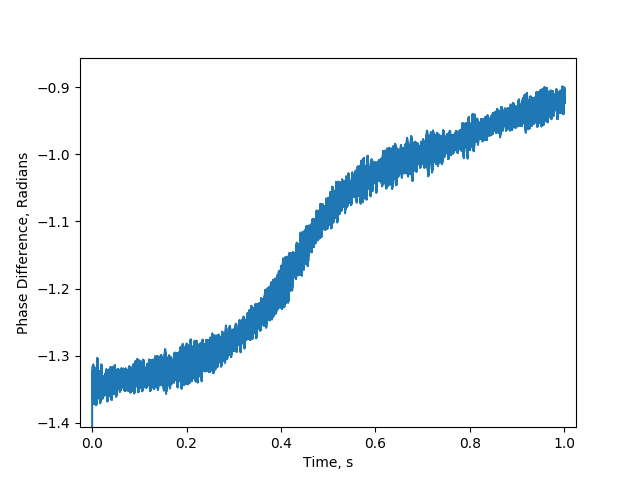
\includegraphics[width=0.9\textwidth, center,angle=0]{DImages/Phase_Difference_shot_2_Date_20180411.png}
\caption{Shot 2 taken on 11-04-2018 on the Koheron laser shows that a drift of 0.4 Rad is present. This also has 2 distinctive turning points in phase difference.}
\label{fig:PD-shot-2-20180411}
\end{figure}

Shots taken around this time show a very large amount of phase noise at varying bandwidths. It is believed that this is caused by a mismatch in path length between interfering paths within the interferometer. As can be seen in the difference between the two different sets of phase noise plots shown in \autoref{fig:2-PN-shot-2-20180323-bw-1000-40000-unmatched} and \autoref{fig:2-PN-shot-2-20180323-bw-1000-40000-matched} which have unmatched and matched path lengths respectively. The result of matching the path lengths is very significant, as the total path length is 7m, this means the addition of 1/7th of the total path length resulted in a reduction in phase noise of two thirds.
\begin{figure}
  \begin{subfigure}{.5\textwidth}
    \centering\captionsetup{width=.9\linewidth}
    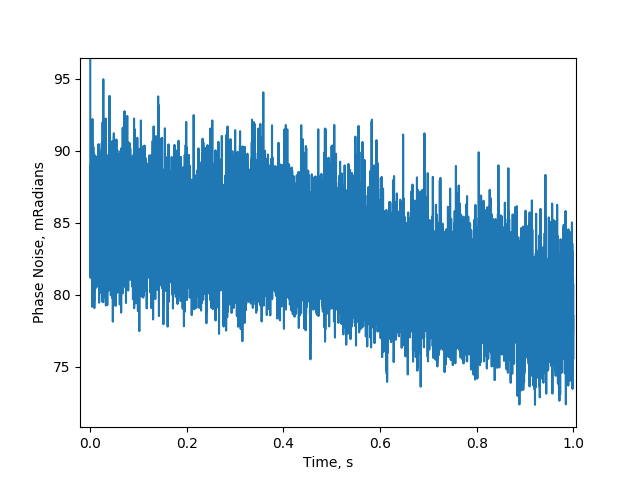
\includegraphics[width=\textwidth,angle=0]{DImages/Phase_Noise_for_Scene_shot_2_with_bandwidth___1000_Date_20180323.png}
    \caption{Phase noise graph at a bins of 1000 therefore a bandwidth of 20KHz.}
  \end{subfigure}
  \begin{subfigure}{.5\textwidth}
    \centering\captionsetup{width=.9\linewidth}
    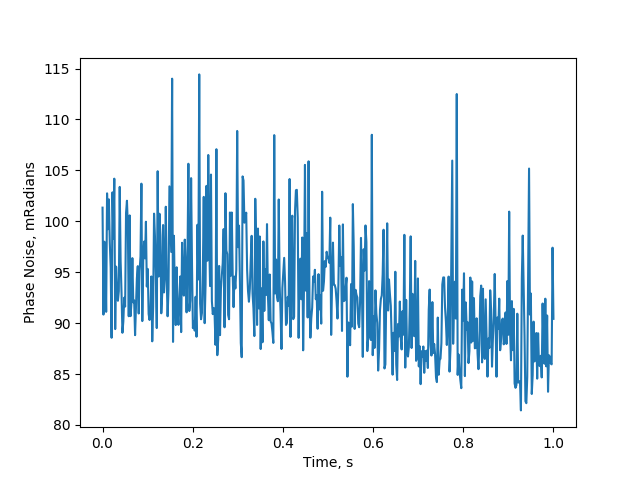
\includegraphics[width=\textwidth, angle=0]{DImages/Phase_Noise_for_Scene_shot_2_with_bandwidth___40000_Date_20180323.png}
    \caption{Phase noise graph at a bins of 40000 therefore a bandwidth of 500Hz}
  \end{subfigure}
\caption{Phase noise of Shot 2 taken on 23/03/18 at two different bandwidths. Length of scene interferometer arm miss matched by ~1m. Bandwidth of 500Hz on figure (b) shows a large amount of structure due to the fact it is likely being performed over some turning points.}
\label{fig:2-PN-shot-2-20180323-bw-1000-40000-unmatched}
\end{figure}

\begin{figure}
  \begin{subfigure}{.5\textwidth}
    \centering\captionsetup{width=.9\linewidth}
    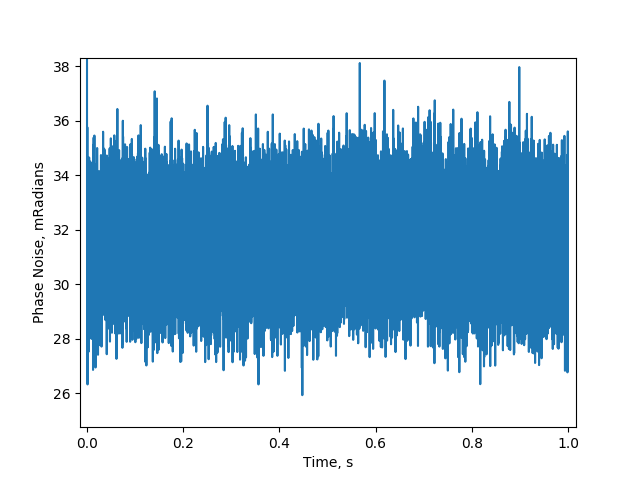
\includegraphics[width=\textwidth,angle=0]{DImages/Phase_Noise_for_Scene_shot_8_with_bandwidth___1000_Date_20180323.png}
    \caption{Phase noise graph at a bins of 1000 therefore a bandwidth of 20KHz.}
  \end{subfigure}
  \begin{subfigure}{.5\textwidth}
    \centering\captionsetup{width=.9\linewidth}
    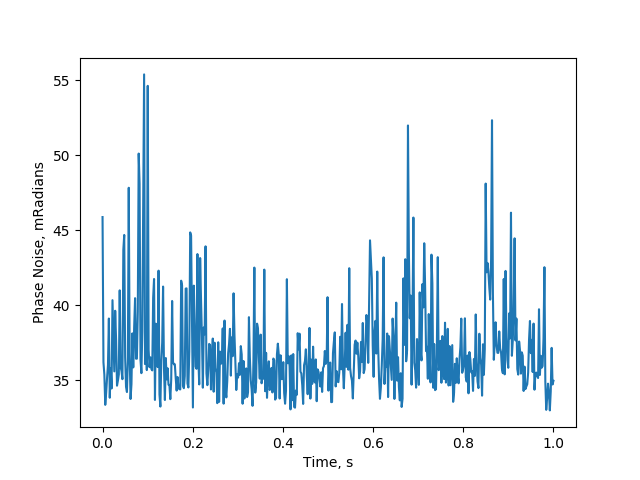
\includegraphics[width=\textwidth, angle=0]{DImages/Phase_Noise_for_Scene_shot_8_with_bandwidth___40000_Date_20180323.png}
    \caption{Phase noise graph at a bins of 40000 therefore a bandwidth of 500Hz}
  \end{subfigure}
\caption{Phase noise of Shot 8 taken on 23/03/18 at two different bandwidths. Length of scene interferometer arms are now matched to within 1cm. Bandwidth of 500Hz on figure (b) shows a large amount of structure due to the fact it is likely being performed over some turning points.}
\label{fig:2-PN-shot-2-20180323-bw-1000-40000-matched}
\end{figure}

\begin{figure}[H] 
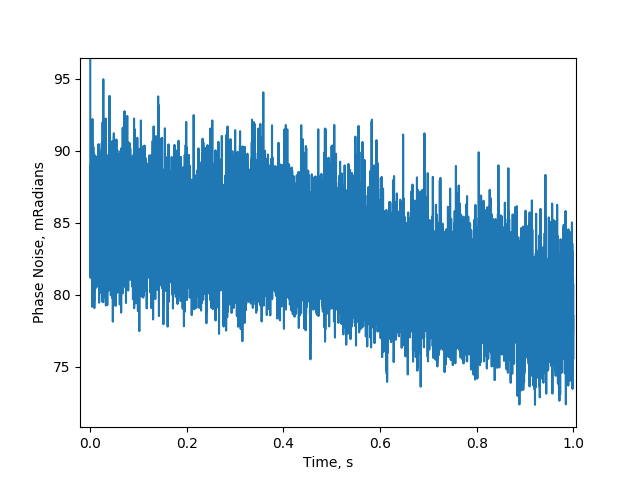
\includegraphics[width=0.9\textwidth, center,angle=0]{DImages/Phase_Noise_for_Scene_shot_2_with_bandwidth___1000_Date_20180323.png}
\caption{Phase noise graph at a bins of 1000 therefore a bandwidth of 20KHz}
\label{fig:PN-shot-2-20180323-bw-1000}
\end{figure}

\begin{figure}[H] 
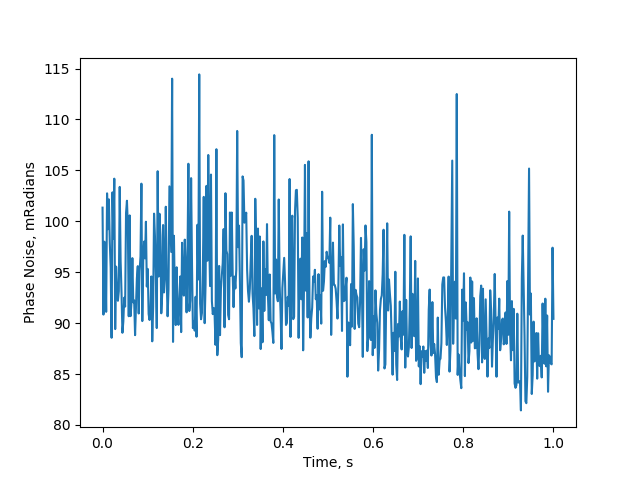
\includegraphics[width=0.9\textwidth, center,angle=0]{DImages/Phase_Noise_for_Scene_shot_2_with_bandwidth___40000_Date_20180323.png}
\caption{Phase noise graph at a bins of 40000 therefore a bandwidth of 500Hz}
\label{fig:PN-shot-2-20180323-bw-40000}
\end{figure}

%----------------------------------------------------------------------------------------
%	New Laser
%----------------------------------------------------------------------------------------
\chapter{New Laser}

%----------------------------------------------------------------------------------------
%	Results
%----------------------------------------------------------------------------------------
\section{Overview and Operation}
The new laser, which is an SFL1550S from Thorlabs \cite{ThorlabsFC/APC} has many advantages over the Koheron based laser system. As shown by the specification it does have regions of multi mode operation between 75-125mA and 250 to 300 mA as shown by \autoref{fig:Multimodelaser}. As a result the chosen operating current is $185 \pm 0.01$ mA, which results in approximately 30mW of output power. The linewidth of this laser is typically 50 KHz but can display a max linewidth of 100KHz. In a worst case scenario this is an improvement of factor 60 over the linewidth of the Koheron based system. In addition to this by operating this laser via the laser driver \cite{CompactPackages}, also from thorlabs, the laser can also be temperature controlled to a precision of $\pm 0.01K$. The heating of the laser cavity can cause emission of undesired photons by increasing the linewidth and can also disturb the coherence of the phase that results in an increase of phase noise. By temperature controlling the laser and therefore the cavity, this process can be minimised resulting in cleaner signal with the narrowest linewidth possible.

\begin{figure}[H] 
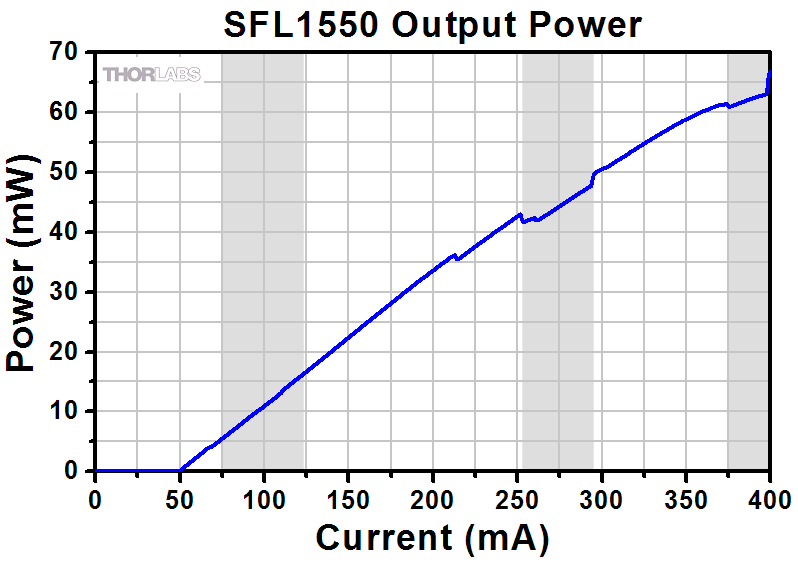
\includegraphics[width=0.85\textwidth, center,angle=0]{DImages/Multimodelaser.PNG}
\caption{Shows the relationship between operating current and output power of the laser. The greyed areas are regions in which multimode operation occurs \cite{ThorlabsFC/APC}.}
\label{fig:Multimodelaser}
\end{figure}

\section{Results}

Initial tests with the new laser at 185mA have shown vast improvements over that of the old system. With phase noise consistently at a value of 3mRad or less at a bandwidth of 20KHz which can be seen by \autoref{fig:4-shot-26-20180416} (c). The same set of plots also shows all of the important parameters to establish the characteristics of the laser. It shows that drift is still present, which solidifies hypothesis about the temperature variations in the fiber optics being a primary cause for the movement of phase. Since the phase noise is now reduced many more phase variations can be seen within the signal, which is important as this mimics certain variations in plasma density which would also only be able to seen if the phase noise is sufficiently low, e.g. sawtooth instabilities.

\begin{figure}[H]
  \begin{subfigure}{.5\textwidth}
    \centering\captionsetup{width=.9\linewidth}
    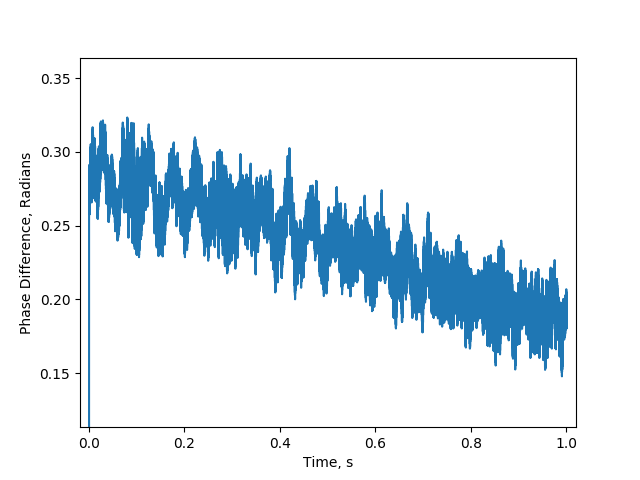
\includegraphics[width=\textwidth,angle=0]{DImages/Phase_Difference_shot_26_Date_20180416.png}
    \caption{Phase difference with the new laser. Drift is still significant, but with reduced phase noise small variations in phase difference can now be seen as they were likely previously swamped out by noise.\\}
  \end{subfigure}
  \begin{subfigure}{.5\textwidth}
    \centering\captionsetup{width=.9\linewidth}
    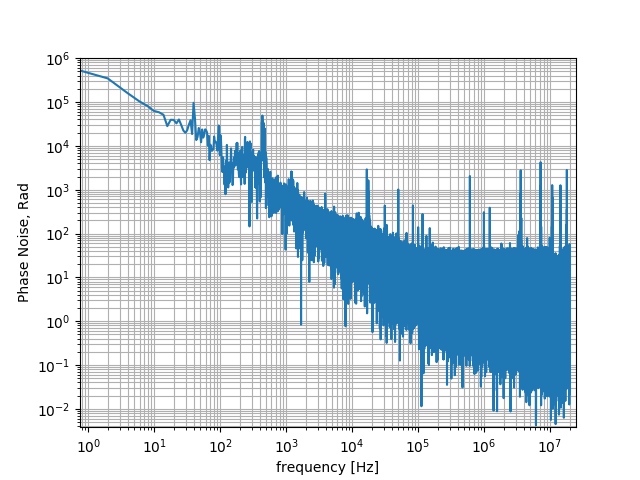
\includegraphics[width=\textwidth, angle=0]{DImages/FFT_for_shot_26_Date_20180416.png}
    \caption{FFT shows single mode operation as expected by running at 185mA. Level of white noise is around 35 Rad which is an order of magnitude less than seen in FFT's of the Koheron system. The low frequency noise remains unchanged.}
  \end{subfigure}
  \begin{subfigure}{.5\textwidth}
    \centering\captionsetup{width=.9\linewidth}
    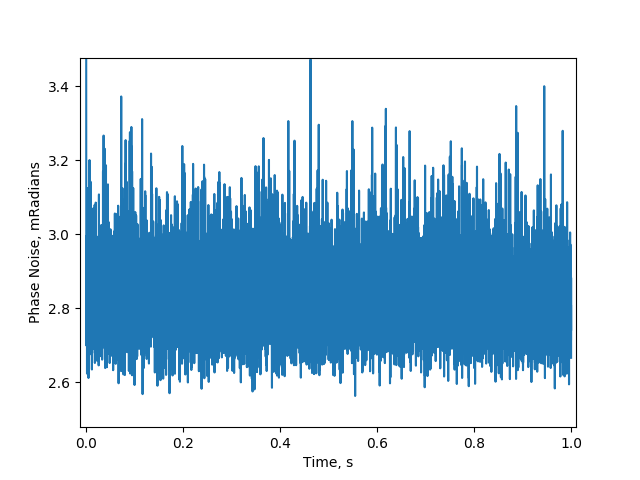
\includegraphics[width=\textwidth,angle=0]{DImages/Phase_Noise_for_Scene_shot_26_with_bandwidth___1000_Date_20180416-1.png}
    \caption{Phase noise graph at a bins of 1000 therefore a bandwidth of 20KHz.}
  \end{subfigure}
  \begin{subfigure}{.5\textwidth}
    \centering\captionsetup{width=.9\linewidth}
    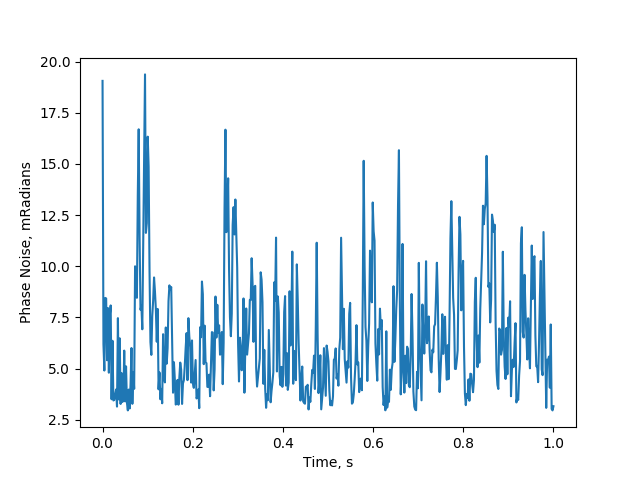
\includegraphics[width=\textwidth, angle=0]{DImages/Phase_Noise_for_Scene_shot_26_with_bandwidth___40000_Date_20180416.png}
    \caption{Phase noise graph at a bins of 40000 therefore a bandwidth of 500Hz}
  \end{subfigure}
\caption{Data gathered for shot 26 taken on 16/04/18. Shows that the new laser has given significant improvements to different parameters of the system including a phase noise of 3 mRad at 20KHz bandwidth.}
\label{fig:4-shot-26-20180416}
\end{figure}

The interferometer is also sensitive to external vibrations that cause an oscillation in the retroreflector. This can be seen clearly in \autoref{fig:2-modulating-vib} by applying a vibrating speaker to the translation stage. It can be seen by analysing the FFT that by inducing a 100Hz signal many other signals close to that frequency can also be detected. The same effect is also seen when the optical bench is tapped lightly which is shown in \autoref{fig:PD-shot-14-20180416-zoomedplot}. When the table is tapped the signal produced is quickly damped and this can be seen on the large scale plot. The zoomed plot shows that within the low frequency signal caused by the tap a higher frequency signal is also seen. 

\begin{figure}[H]
  \begin{subfigure}{.5\textwidth}
    \centering\captionsetup{width=.9\linewidth}
    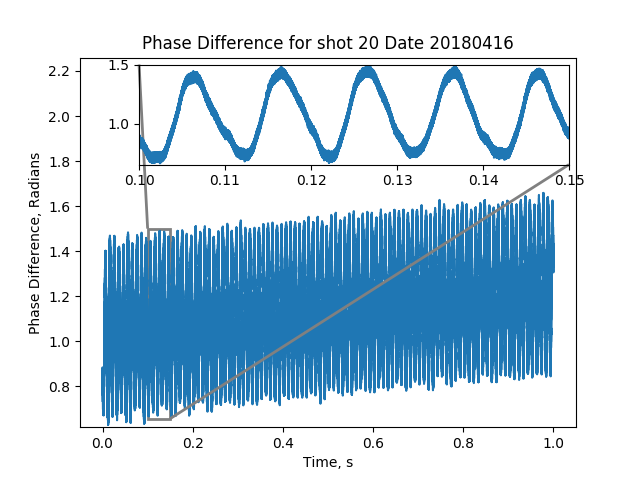
\includegraphics[width=\textwidth,angle=0]{DImages/PD_-_shot_20_-_20180416_-_zoomed_plot_-_100Hz_speaker.png}
    \caption{While taking a shot when a vibrating speaker was outputting 100Hz a zoomed in small cross section in the x-axis shows that this signal is actually an oscillation of approximately 100Hz}
  \end{subfigure}
  \begin{subfigure}{.5\textwidth}
    \centering\captionsetup{width=.9\linewidth}
    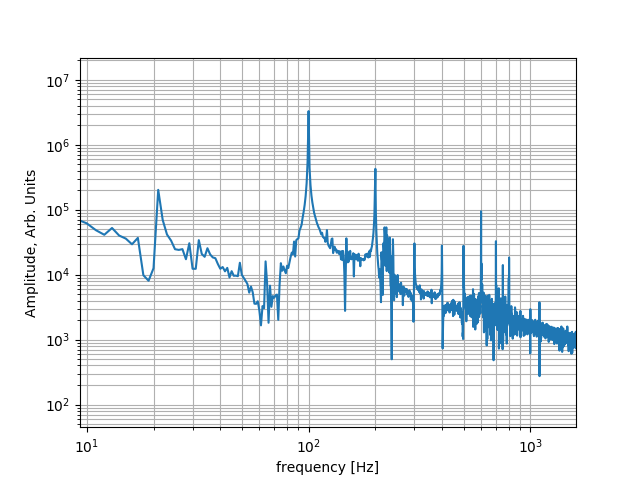
\includegraphics[width=\textwidth, angle=0]{DImages/FFT_for_shot_20_Date_20180416.png}
    \caption{FFT of the shot reveals that while there is a frequency spike at 100Hz this also has a linewidth and is surrounded by a few other frequencies, likely harmonics to the 100Hz. The linewidth is visible as phase noise.}
  \end{subfigure}
\caption{Shot 20 taken on 16-04-2018 where a vibrospeaker has been placed next to the retroreflector and is operated at 100Hz. This frequency can clearly be seen within both plots and shows that the signal is being represented effectively.}
\label{fig:2-modulating-vib}
\end{figure}

\begin{figure}[H] 
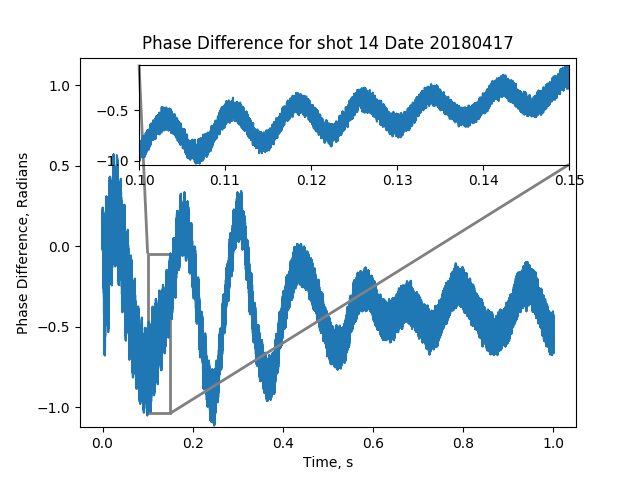
\includegraphics[width=0.9\textwidth, center,angle=0]{DImages/Shot_14_20180417_Zoom_Plot.png}
\caption{Tapping the table results in a low frequency oscillation that also has higher frequencies mixed in. This is important for the system as this will represent the mechanical vibrations occuring, seeing that they only cause an oscillation is good as this will not effect the density calculation and will be cancelled out when the oscillation is seen on both the HeNe and 1550nm laser.}
\label{fig:PD-shot-14-20180416-zoomedplot}
\end{figure}

\subsection{Separating Scene and Reference Signals}

In order to further analyse to the contribution of drift by each of the interferometer arms a new interferometer set up was devised which is shown in \autoref{fig:intconfig4}. The benefit of this set up is that the signal from each interferometer, scene and reference, is compared to that of the driving frequency of the AOM. This should allow the viewing of which path is contributing more to the drift of the phase difference. If both paths were to drift equally, this would be cancelled out and wouldn't matter in the calculation as this was the intention of using an interferometer as the reference signal rather than the function generator. If the interferometer is working as expected and the drift is a function of pressure and temperature changes along the portion of free space then the reference should show a constant drift and the scene should be a modulated form of the reference signal where the modulation is provided by temperature and pressure changes in the free space. This was achieved by modifying the code in the SPEC board to allow signals from four lots of 1550nm signals rather than 2 1550nm and 2 HeNe signals, like would be used in the final system.

From analysing the data shown in \autoref{fig:2-2ch-scene-ref} the scene and the reference drift the result is quite confusing. The phase of each of the channels appears to diverge at t=0.6s. Since the comparison signal is identical for both phase calculation this implies the phase in each interferometer is moving in an opposite direction. This can only be explained by two different scenarios; the free space portion of the scene interferometer experiences a temperature or pressure change that reflects the turning point at t=0.4s, or the temperature in the fiber optics of each interferometer path is slightly different.

\begin{figure}[H]
  \begin{subfigure}{.5\textwidth}
    \centering\captionsetup{width=.9\linewidth}
    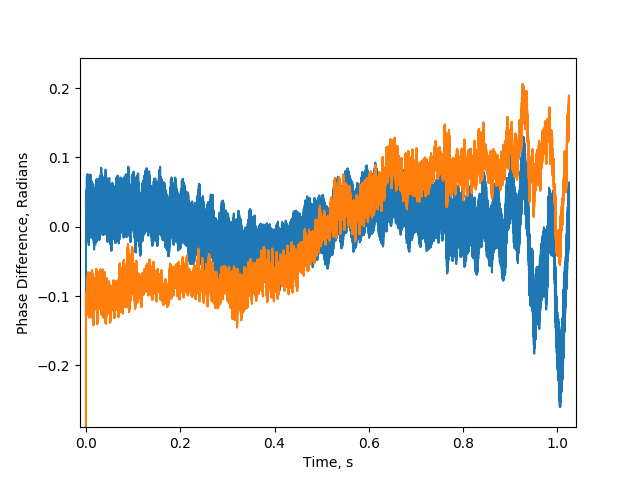
\includegraphics[width=\textwidth,angle=0]{DImages/Phase_Difference_Blue___Scene_Orange___Reference_shot_9_Date_20180417.png}
    \caption{Individual phase drift of each interferometer as the raw signal at 20MS/s \\}
  \end{subfigure}
  \begin{subfigure}{.5\textwidth}
    \centering\captionsetup{width=.9\linewidth}
    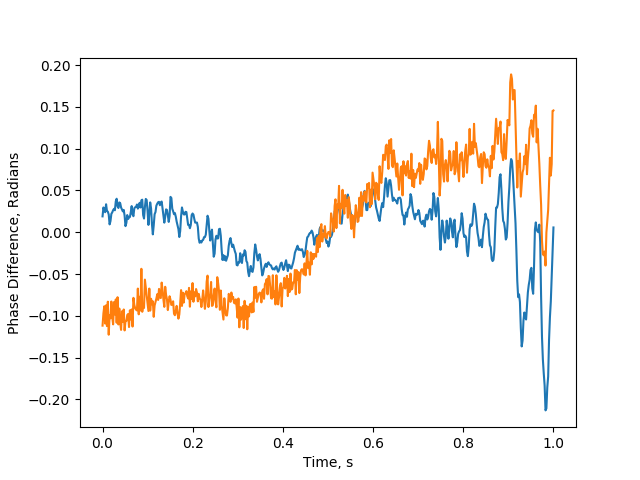
\includegraphics[width=\textwidth, angle=0]{DImages/avr_2ch_shot_9_20180417.png}
    \caption{Signal has been averaged into 500 bins to show underlying structure and magnitude of drift.}
  \end{subfigure}
\caption{Shot 9 taken on 17-04-2018 where the scene and reference interferometers have a phase difference calculation compared to the same signal that is driving the AOM. In both plots the blue data represents the scene interferometer and the orange represents the reference interferometer.}
\label{fig:2-2ch-scene-ref}
\end{figure}


%----------------------------------------------------------------------------------------
%	Conclusion
%----------------------------------------------------------------------------------------
\chapter{Conclusion}
\section{Phase Noise}
Overall the phase noise of the system can be said to be consistently low enough to fit the specified criterion. The phase noise has slight variations based on factors such as temperature in the room, current supplied to the laser and whether vibrations are sufficiently damped. As can be seen in \autoref{fig:4-phase-noise} the noise is consistently achieved at a value of 3mRad or bellow across a number of shots, using the new laser. This shows a vast improvement over the Koheron system (A consistent factor of 4 improvement along with a increase in stability) and is now comparable to the precision given by the CO2 system currently installed on MAST-U. Using the new laser average value of $3.025 \pm 0.065 mRad$ between the 4 plots seen in \autoref{fig:4-phase-noise} this would represent a density change in the plasma of $~ 6.07\times 10^{17} \pm 2.06\times 10^{17} m^{2}$

\begin{figure}[H] 
  \begin{subfigure}{.5\textwidth}
    \centering\captionsetup{width=.9\linewidth}
    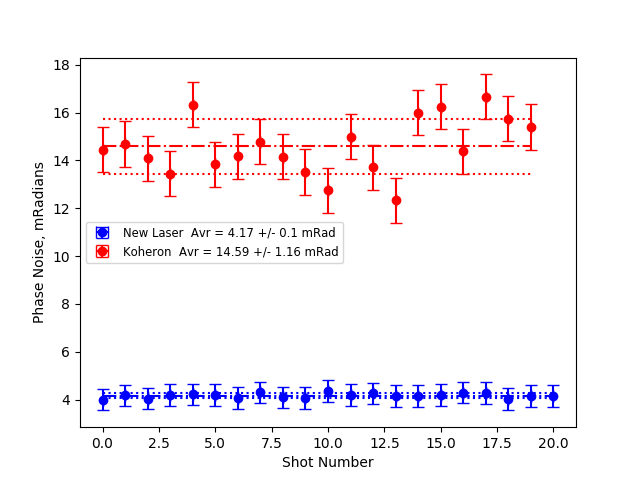
\includegraphics[width=\textwidth, angle=0]{DImages/Phase_Noise_for_Shots_1and_2.png}
    \caption{New Laser consists of shots 1-20 and Koheron consists of shots 21-40.}
  \end{subfigure}
  \begin{subfigure}{.5\textwidth}
    \centering\captionsetup{width=.9\linewidth}
    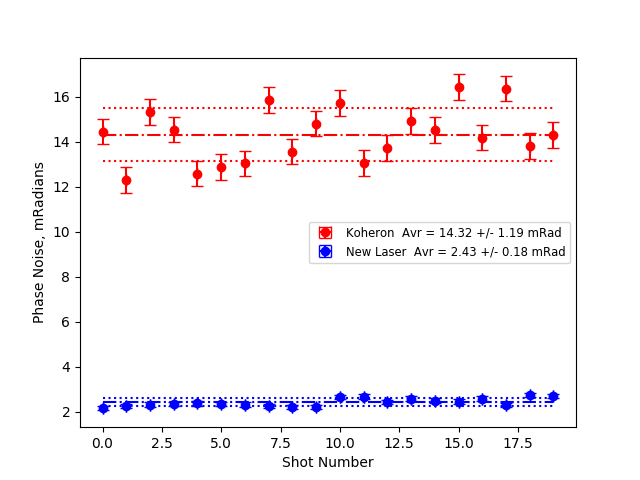
\includegraphics[width=\textwidth, angle=0]{DImages/Phase_Noise_for_Shots_3and_4.png}
    \caption{New Laser consists of shots 61-80 and Koheron consists of shots 41-60.}
  \end{subfigure}
  \begin{subfigure}{.5\textwidth}
    \centering\captionsetup{width=.9\linewidth}
    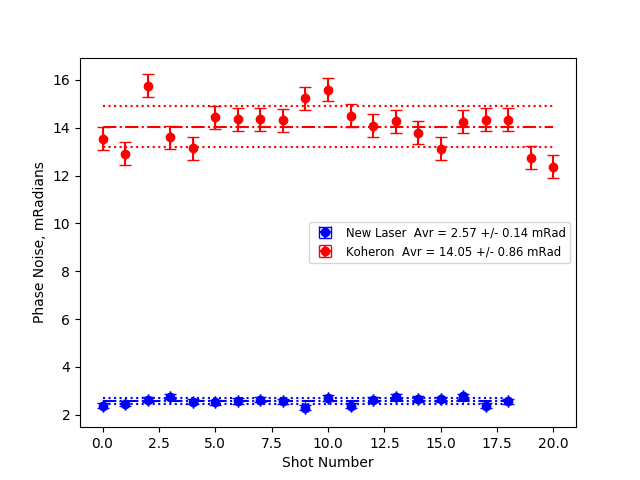
\includegraphics[width=\textwidth,angle=0]{DImages/Phase_Noise_for_Shots_5and_6.png}
    \caption{New Laser consists of shots 81-100 and Koheron consists of shots 106-125.}
  \end{subfigure}
  \begin{subfigure}{.5\textwidth}
    \centering\captionsetup{width=.9\linewidth}
    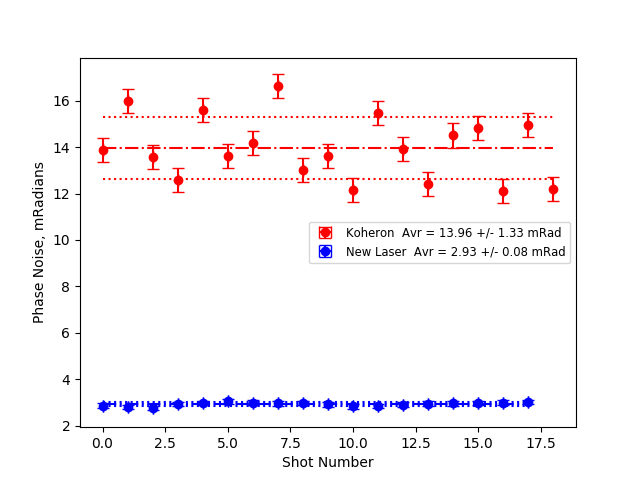
\includegraphics[width=\textwidth, angle=0]{DImages/Phase_Noise_for_Shots_7and_8.png}
    \caption{New Laser consists of shots 146-165 and Koheron consists of shots 126-145.}
  \end{subfigure}
\caption{Collection of shots all taken on the same day (23/04/2018) within an hour showing the variation in the phase noise between identical conditions with the only variable factor being the laser. In all plots blue data represents the use of the New laser and red data represents the use of the Koheron laser. (a) shows shots with no insulation. (b) shows shots with insulation present. (c) shows shots with copper tape adding thermal mass but no insulation. (d) shows shot with copper tape and insulation.}
\label{fig:4-phase-noise}
\end{figure}

\section{Phase Drift}
Using the equation for the refractive index of air with varying pressure and temperature:

\begin{equation}
n(P, T) = (1 + 0.000293 \times \frac{P}{P_{0}} \frac{T_{0}}{T})\times 0.4
\label{eq:refractive-temp}
\end{equation}

Where $\frac{P}{P_0} = 1$ therefore assuming air pressure change is negligible. $T_0 = 295K$ as standard room temperature is 22 degrees. T is the temperature change that contributes to the change in refractive index. And the 0.4 is due to the 0.2m double pass free space portion of the interferometer. Using a temperature change of 0.5 degrees \cite{Melikov1997AirRooms} this results in a path difference of $\pm 198\times 10^{-9}m$ which would result in a phase change of $\pm 0.8 Radians$. This number is within the scope of the drift we expect to see, however this assumes that the whole free space portion changes by this amount. Combining this with the fact that the pressure may also change, this is a cause for concern in our final measurement.

Equally if we consider the fiber optics as a contributing component to this shift using the refractive index of 1550nm fiber $n_{0} - 1.4681$ the same temperature change will result in a change of phase of $\pm 20000 Radians$. From this simple calculation we see that the shift due to the free space is negligible compared the the shift in fiber. From this we can say that the temperature shift in fiber is of the order of $\pm 10^{-5} Degrees Kelvin$ to produce a phase shift of 0.4 Radians. It is worth noting that this equation also should have a function of time to it, as we see this shift over the course of a 1 second shot. If the temperature response is sufficiently slow it will be damped greatly on the scale of the shot length, this is likely why we only see a 0.4 Radian drift rather than 20000 Radians. The ratio between these refractive indices already shows that the sensitivity of temperature in fiber is on the order of 1600x greater.

It has been found that the drift that is caused by temperature changes within the fiber is a major issue with the system. Fiber optic interferometers have been designed where their primary purpose is measurement of temperature \cite{Hocker1979Fiber-opticTemperature}. The paper discusses that with a Helium Neon fiber optic system it is common to see phase drifts of the order of over 100 radians per degree C per meter. Since we require precisions that are many orders of magnitude lower than this it is unlikely a level of sufficient temperature control can be achieved. The phase drift is unpredictable and ultimately limits the resolution of the system to the value of the drift as a result this massively increases the errors on the calculated density of the plasma. As is seen in \autoref{fig:4-max-min-drifts} the drift is wildly inconsistent between shots taken under exact conditions with very little time between shots. The only thing that can be said with confidence is that on average the new laser reduces the amount of drift seen, and insulation also reduces the variance in the drift. The insulation used was a combination of bubble wrap and foam, which showed general reduction in drift visible on an oscilloscope. However replacing this with house insulation didn't seem to show any signs of improvement. This is likely because we are the limits of how much insulation can reduce the temperature fluctuations in the fiber optic cables.

\begin{figure}[H] 
  \begin{subfigure}{.5\textwidth}
    \centering\captionsetup{width=.9\linewidth}
    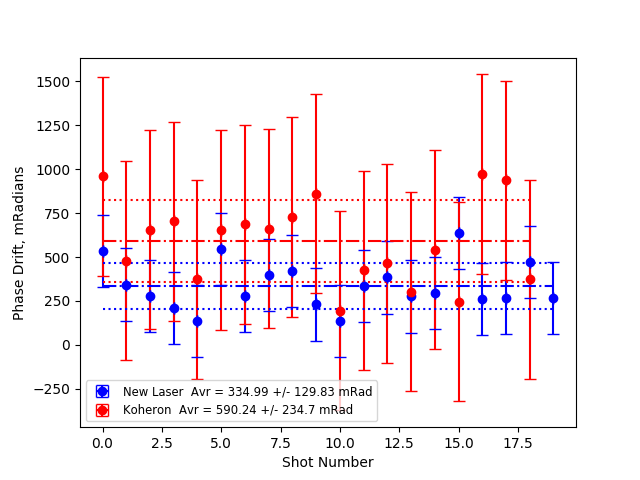
\includegraphics[width=\textwidth, angle=0]{DImages/Max_-_Min_Drift_for_Shots_1and_2.png}
    \caption{New Laser consists of shots 1-20 and Koheron consists of shots 21-40.}
  \end{subfigure}
  \begin{subfigure}{.5\textwidth}
    \centering\captionsetup{width=.9\linewidth}
    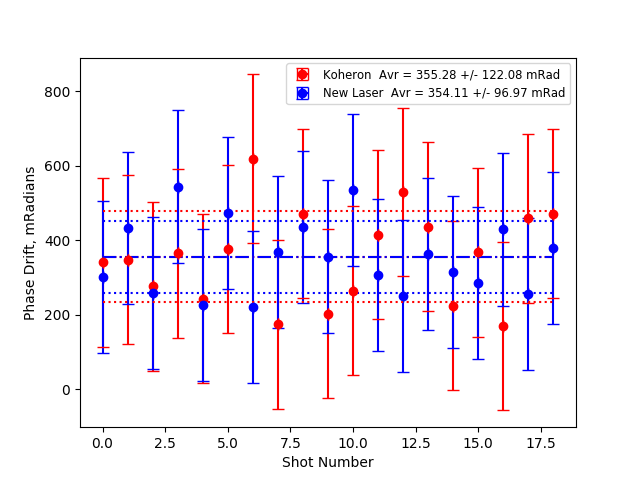
\includegraphics[width=\textwidth, angle=0]{DImages/Max_-_Min_Drift_for_Shots_3and_4.png}
    \caption{New Laser consists of shots 61-80 and Koheron consists of shots 41-60.}
  \end{subfigure}
  \begin{subfigure}{.5\textwidth}
    \centering\captionsetup{width=.9\linewidth}
    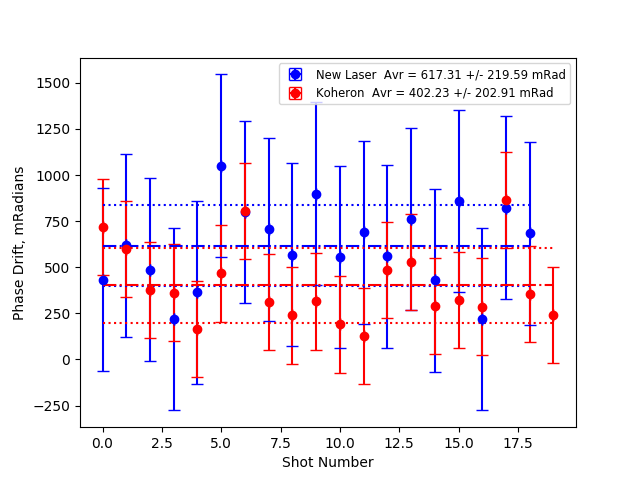
\includegraphics[width=\textwidth,angle=0]{DImages/Max_-_Min_Drift_for_Shots_5and_6.png}
    \caption{New Laser consists of shots 81-100 and Koheron consists of shots 106-125.}
  \end{subfigure}
  \begin{subfigure}{.5\textwidth}
    \centering\captionsetup{width=.9\linewidth}
    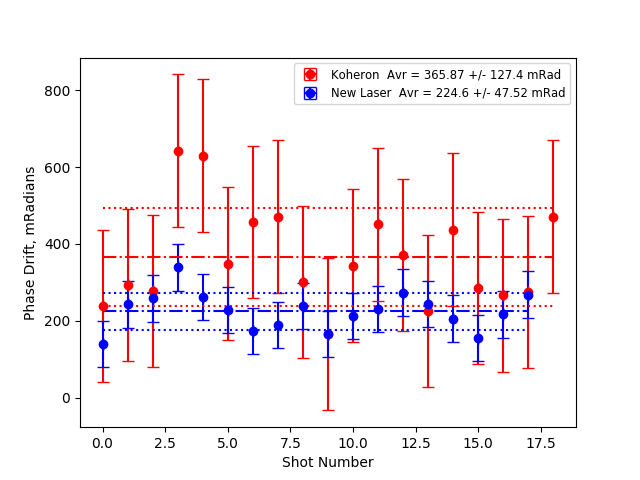
\includegraphics[width=\textwidth, angle=0]{DImages/Max_-_Min_Drift_for_Shots_7and_8.png}
    \caption{New Laser consists of shots 146-165 and Koheron consists of shots 126-145.}
  \end{subfigure}
\caption{Collection of shots all taken on the same day (23/04/2018) within an hour showing the variation in the phase drift between identical conditions with the only variable factor being the laser. In all plots blue data represents the use of the New laser and red data represents the use of the Koheron laser. (a) shows shots with no insulation. (b) shows shots with insulation present. (c) shows shots with copper tape adding thermal mass but no insulation. (d) shows shot with copper tape and insulation.}
\label{fig:4-max-min-drifts}
\end{figure}
%----------------------------------------------------------------------------------------
%	Discussion
%----------------------------------------------------------------------------------------


%----------------------------------------------------------------------------------------
%	Bibliography
%----------------------------------------------------------------------------------------
\pagebreak
\chapter{Bibliography}
	\printbibliography[heading=none]

\pagebreak

%----------------------------------------------------------------------------------------
%	Appendix
%----------------------------------------------------------------------------------------

\pagenumbering{roman}
\setcounter{page}{2}
\chapter{Appendix}
\begin{appendices}

%\includepdf[pages={ - }]{ChristopherHicklingSummerProject.pdf}
\section{Python Analysis Code}
	%\lstinputlisting[language=Python]{Code/chickling_additions_2.py}
	%\label{chickling_additions}

\end{appendices}

\end{document}